%\documentclass[german,bachelor]{swsLeipzig}
\documentclass[german,bachelor]{swsLeipzig}
% When you change the language, pdflatex may halt on recompilation.
% Just hit enter to continue and recompile again. This should fix it.

%
% Values
% ------
\ThesisSetTitle{Ermittlung von Konfigurationsoptionen im Source Code mit Fokus auf Machine Learning Bibliotheken in Python}
\ThesisSetKeywords{These, Are, My keywords} % only for PDF meta attributes

\ThesisSetAuthor{Marco Jaeger-Kufel}
\ThesisSetStudentNumber{3731679}
\ThesisSetDateOfBirth{10}{05}{1995}
\ThesisSetPlaceOfBirth{Hannover}

\ThesisSetSupervisors{Prof.\ Dr.\ Norbert Siegmund, Sebastian Simon{,} M.Sc.}

\ThesisSetSubmissionDate{14}{06}{2022}

%
% Suggested Packages
% ------------------
\usepackage[sort&compress]{natbib}
%   Allows citing in different ways (e.g., only the authors if you use the
%   citation again within a short time).
%
\usepackage{booktabs}
%    For tables ``looking the right way''.
%
%\usepackage{tabularx}
%    Enables tables with columns that automatically fill the page width.
%
%\usepackage[ruled,algochapter]{algorithm2e}
%    A package for pseudo code algorithms.
%
%\usepackage{amsmath}
%    For tabular-style formatting of mathematical environments.
%

%
% Commenting (by your supervisor)
% -------------------------------
\usepackage{xcolor}
\usepackage{soul}
\usepackage{listings}
\usepackage{multirow}
\usepackage[euler]{textgreek}
\usepackage{graphicx}
\usepackage{lscape}
\usepackage{makecell}
\newcommand{\bscom}[2]{%
  % #1 Original text.
  % #2 Replacement text.
    \st{\scriptsize\,#1}{\color{blue}\scriptsize\,#2}%
  }

% Create links in the pdf document
% Hyperref has some incompatibilities with other packages
% Some other packages must be loaded before, some after hyperref
% Additional options to the hyperref package can be provided in the braces []
\usehyperref[backref] % This will add back references in the bibliography
\usepackage[utf8]{inputenc}
\usepackage{textcomp}
\usepackage{tikz,pgfplots}
\usetikzlibrary{shapes.geometric, arrows}
\usetikzlibrary{patterns}
\usepackage{float}
%\setcitestyle{authoryear,close={)}}
%\setcitestyle{author}

\begin{document}
\begin{frontmatter}
  \begin{abstract}
      Über Konfigurationsoptionen können die Nutzenden eine Software an ihre Bedürfnisse anpassen.
      Die Wahl der Konfigurationsoptionen hat dabei einen kritischen Einfluss auf die Ausführung des Source Codes.
      Gleichzeitig bleiben Konfigurationsfehler oft unentdeckt oder sind schwer nachzuvollziehen.
      Im Machine Learning (ML) Bereich liegen Konfigurationsoptionen in Form von Hyperparametern vor,
      mit denen ML-Algorithmen, beispielsweise das Trainieren eines Modells, gesteuert werden können.
      Es gibt jedoch keine Übersicht darüber, wie ML-Algorithmen konfiguriert werden.
      Diese Arbeit stellt einen Ansatz vor, bei dem ML-Konfigurationsoptionen in Python Source
      Code extrahiert werden können.
      Mittels statischer Code-Analyse lassen sich mit diesem Ansatz die Konfigurationsoptionen populärer ML-Bibliotheken
      in beliebigen Softwaresystemen lokalisieren.
      Darüber hinaus können mit Hilfe von Techniken aus der Datenflussanalyse auch bei variablen Hyperparametern
      mögliche Konfigurationswerte bestimmt werden.
      Mit dem Ansatz können so ML-Algorithmen und die Konfigurationsoptionen mit einer sehr hohen Genauigkeit identifiziert
      werden.

  \end{abstract}

  \tableofcontents

  %\chapter*{Acknowledgements} % optional
  %I thank the authors of the swsLeipzig template for their excellent work!

  \listoffigures % optional
  \addcontentsline{toc}{chapter}{\listfigurename}
  \listoftables % optional
  \addcontentsline{toc}{chapter}{\listtablename}
  %\addcontentsline{toc}{chapter}{Listings}
  %\lstlistoflistings \label{Listings}
  %\listofalgorithms % optional
  %    requires package algorithm2e

  % optional: list of symbols/notation (e.g., using the nomencl package)
\end{frontmatter}

\chapter{Einleitung}\label{Einleitung}
%Diese Arbeit entsteht am Institut für Informatik an der Universit\"at Leipzig in der Abteilung \glqq Softwaresysteme\grqq.
%Im Folgenden wird die zugrundeliegende Problemstellung und Relevanz erl\"autert.
%Anschlie\ss end wird dieses Problem auf einen konkreten Anwendungsbereich \"ubertragen und auf die Zielsetzung der Arbeit eingegangen.\\

\section{Motivation}
Moderne Softwaresysteme ermöglichen den Nutzenden ein breites Spektrum unterschiedlicher Konfigurationsoptionen.
Anhand dieser Konfigurationsoptionen sind die Nutzenden in der Lage, die Ausführung einer Software zu steuern, zum Beispiel
hinsichtlich der Performance oder Funktionalität \cite[]{10.1145/3427921.3450255}.
Konfigurationsoptionen können dabei ganz unterschiedliche Funktionen besitzen, die von den Nutzenden nach den eigenen Bedürfnissen angepasst werden können.\\
\indent Konfigurationsoptionen können in verschiedenen Teilen eines Softwareprojekts verarbeitet, definiert und beschrieben werden,
wie beispielsweise in den Konfigurationsdateien, im Source Code und in der Dokumentation \cite[]{7774519}.
Sie werden meist als Key-Value Pair entworfen und gesammelt in einer Konfigurationsdatei gespeichert.
Dem Namen der Konfigurationsoption (Key) werden dabei Einstellungsmöglichkeiten beliebigen Typs zugeordnet (Value).
Ein einheitliches Schema zur Speicherung von Konfigurationsdateien gibt es jedoch nicht, weshalb sich diese
von der Struktur und Syntax unterscheiden \cite[]{10.1145/1985793.1985812}.\\
\indent In Softwaresystemen aus dem Machine Learning Bereich sind Konfigurationsoptionen im Source Code
in Form von sogenannten \textit{Hyperparametern} vorhanden.
Machine Learning (ML) ist ein Teilgebiet der künstlichen Intelligenz, in der die Art und Weise, wie Menschen lernen,
imitiert wird.
Durch den Einsatz statistischer Methoden werden Algorithmen trainiert, um beispielweise Klassifizierungen oder Vorhersagen
zu treffen.
Bei Hyperparametern handelt es sich um Parameter eines Machine Learning Algorithmus,
die vor Beginn des Lernprozesses vom Nutzenden festgelegt werden können.
Sie werden als Parameter an die jeweilige Klasse übergeben und bieten den Nutzenden Konfigurationsmöglichkeiten für
das Training des Modells \cite[]{hype}.\\
\indent Die Zahl der Machine Learning Anwendungen ist in den letzten Jahren stark gestiegen.
Unter anderem durch den Erfolg und den Möglichkeiten des Internets ist nicht nur das Volumen an Daten enorm gewachsen,
auch die Heterogenität der Daten führt dazu, dass herkömmliche Methoden zur Verarbeitung
und Informationsgewinnung nicht mehr ausreichen.
Gleichzeitig trägt die technologische Weiterentwicklung der Rechen- und Speicherleistung von Computern und in den letzten Jahrzehnten dazu bei,
dass durch neue Ansätze des Machine Learnings die rasant wachsenden Datenmengen leistungsfähig verarbeitet werden können \cite[]{FRADKOV20201385}.\\
\indent Dennoch fehlt es in der Forschung an Ansätzen, um Konfigurationsoptionen von ML Algorithmen zu lokalisieren und extrahieren.
Weiterhin gibt es keine Übersicht darüber, wie ML Algorithmen konfiguriert werden.
Zudem kann die statische Prüfung der Hyperparameter für den Nutzenden eine Zeitersparnis bedeuten,
wenn sonst ein falscher Konfigurationswert einen langen Batch-Job zum Scheitern bringt
oder das Ergebnis nicht den Erwartungen entspricht. \\

\section{Zielsetzung}
Das Ziel dieser Arbeit ist es, Konfigurationsoptionen im Source Code zu erkennen und zu extrahieren.
Der Fokus liegt hierbei auf die Konfiguration (Hyperparameter) von ML-Algorithmen, die von bekannten ML Bibliotheken
zur Verfügung gestellt werden.\\
\indent Es existieren bereits einige Forschungsansätze zur Ermittlung und Verarbeitung von Konfigurationsoptionen im Source Code.
Viel zitiert wird dabei der Ansatz von \citeauthor{10.1145/1985793.1985812}, den sie \citeyear{10.1145/1985793.1985812} publizierten.
Wie auch \citeauthor{7774519} oder \citeauthor{8049300} entwickelten sie einen Ansatz, mittels statischer Code-Analyse Konfigurationsoptionen
im Source Code zu tracken.
Dabei fokussierten sie sich auf Java, die nach dem TIOBE-Index jahrelang als beliebteste Programmiersprache galt.
Für die Programmiersprache Python, die im Februar 2022 erstmals zur beliebtesten Sprache in diesem Index aufgestiegen seit,
ist diese Thematik jedoch bislang allerdings noch wenig beleuchtet \cite[]{enwiki:1077809155}.
Insbesondere im Bereich des wissenschaftlichen Rechnens (Scientific Computing) gewann Python in den letzten Jahren enorm an Popularität,
weshalb viele Machine Learning Frameworks auf Python basieren \cite[]{2020}.\\
\indent Gegenstand dieser Arbeit sind daher Konfigurationsoptionen von Machine Learning Algorithmen in Python Source Code, die mittels statischer Code-Analyse erkannt werden.
Der Ansatz identifiziert automatisch die Stellen im Source Code, an denen ML-Algorithmen mit Konfigurationsoptionen aus
den zu untersuchenden Bibliotheken gelesen werden und ermittelt für jede dieser Stellen den Namen der Option.
Darauf aufbauend erfolgt eine Datenflussanalyse, um auch für Optionen, die in Form von variablen Parametern übergeben werden,
die möglichen Werte zu ermitteln.
Der Fokus liegt auf drei der populärsten Machine Learning Bibliotheken in Python \cite[]{kaggle}:
\begin{itemize}
 \item TensorFlow
 \item PyTorch
 \item scikit-learn
\end{itemize}
\

\section{Aufbau dieser Arbeit und methodisches Vorgehen}
Im ersten Teil dieser Arbeit wird der theoretische Hintergrund vorgestellt.
Dies umfasst die verwendeten Methoden aus der statischen Code- und Datenflussanalyse, sowie des Web Scrapings.
Zudem erfolgt eine kurze Einführung zu Machine Learning und es wird beschrieben welche Funktionen Python-Bibliotheken und
Konfigurationsoptionen in diesem Zusammenhang erfüllen.
Abgerundet wird der erste Teil mit einer Erläuterung zu Abstract Syntax Trees.
Es folgt ein Exkurs zu den verwandten Arbeiten in Kapitel \ref{Verwandte Arbeiten}.
Im Anschluss wird das methodische Vorgehen des entwickelten Ansatzes in seinen einzelnen Teilschritten von der Auswahl
der Python-Bibliotheken in Abschnitt \ref{choice} bis hin zu der Datenflussanalyse in Abschnitt \ref{dataflow} beschrieben.
Für die Evaluation dieser Arbeit werden die Ergebnisse in Kapitel \ref{Evaluation} zusammengetragen und mit einer manuellen Analyse verglichen.
Diese Ergebnisse werden diskutiert und Limitationen des Ansatzes aufgezeigt, bevor es zum Abschluss noch ein Fazit gibt.

\chapter{Hintergrund}\label{Hintergrund}

\section{Statische Code-Analyse}
Das wichtigste Werkzeug dieser Arbeit ist die statische Code-Analyse,
mit der Software-Projekte unabhängig von der Ausführungsumgebung untersucht werden können.
Bei einer statischen Code-Analyse wird der Quellcode mit computergestützten Methoden untersucht, ohne ihn auszuführen.
Dabei werden die einzelnen Statements im Code anhand der jeweiligen Syntax und Regeln der Programmiersprache analysiert \cite[]{gomes2009overview}.
Die statische Code-Analyse ist ein Werkzeug, um Informationen aus dem Source Code abzuleiten oder
Fehler in einer Softwareanwendung zu reduzieren.
So ermöglichen sie den Anwendenden, alle Pfade des Kontrollflusses der Software zu betrachten oder
Fehler in einem Programm zu finden, die für den Compiler nicht sichtbar sind \cite[]{bardas2010static}.\\
\indent Im Gegensatz zur dynamischen Analyse wird die statische Analyse zur Übersetzungszeit durchgeführt
und setzt damit bereits vor der tatsächlichen Ausführung des Source Codes an.
Die erzeugten Ergebnisse der statischen Analyse lassen sich verallgemeinern, da sie nicht abhängig von den Eingaben sind,
mit denen das Programm während der dynamischen Analyse ausgeführt wurde \cite[]{gomes2009overview}.\\
\indent Für das Aufspüren von Konfigurationsoptionen bietet sich eine statische Code-Analyse daher aus mehreren Gründen an.
So kann es viele Optionen geben, die nur in bestimmten Modulen oder als Folge bestimmter Eingaben verwendet werden.
%Es ist unwahrscheinlich, dass mittels dynamischen Testens alle Verwendungen der gesuchten Konfigurationsoptionen gefunden werden.
%Dies würde zudem bei größeren Softwareprojekten eine sehr komplexe Test-Suite erfordern, um möglichst alle Fälle abdecken zu können.
Gleichzeitig verbergen sich hinter den Methoden und Klassen, der zu untersuchenden Machine Learning Bibliotheken,
teils sehr komplexe und rechenintensive Berechnungen, die bis zu mehreren Tagen laufen können.
Aus Kosten-Nutzen-Überlegungen ist hier eine dynamische Analyse nur bedingt sinnvoll.\\

\section{Datenflussanalyse}
Die Datenflussanalyse ist ein Werkzeug, um Informationen über die möglichen Werte, die an verschiedenen
Stellen in einem Codesegment berechnet werden, zu erfassen.
Es handelt sich um eine statische Analysetechnik mit dem Ziel, das Programmverhalten bereits zur Übersetzungszeit,
also bevor es ausgeführt wird, zu bestimmen.
Der Datenfluss kann mittels eines Kontrollflussgraphens dargestellt werden und Rückschlüsse über das Verhalten des Programms geben.
Der Graph zeigt an, an welchen Stellen eine Variable verwendet wird und welche Werte sie annehmen kann \cite[]{58766}.\\

\noindent Es gibt verschiedene Techniken, die innerhalb der Datenflussanalyse eingesetzt werden, um den Wert von Variablen zu bestimmen.
Eine von ihnen ist \textit{Constant Propagation}.
Das Ziel von Constant Propagation ist es zu bestimmen, an welchen Stellen im Programm eine Variable einen konstanten Wert besitzt.
So kann zum Beispiel toter Code, also redundanter Code, der im weiteren Programmverlauf nicht weiterverarbeitet wird, gefunden werden.
Eine weitere Technik ist \textit{Static Single Assignment}.
Bei dieser Methodik werden die Variablen im Verlauf des Übersetzungsprozesses in eine Zwischenform überführt, in der jede Variable
genau einmal zugewiesen wird.
Die Variablen werden in Versionen aufgeteilt und in der Regel mit einem aufsteigenden Index versehen,
sodass jede Definition ihre eigene Version erhält \cite[]{li2022scalpel}.
Die beiden Techniken Static Single Assignment und Constant Propagation werden in dem statischen Analyse-Framework
\textit{Scalpel} kombiniert \cite[]{li2022scalpel}. \\
\indent Aus dem folgenden Codebeispiel geht hervor, dass die Variable \textit{a} zwei unterschiedliche Werte annehmen kann.\\

\noindent\begin{minipage}{\linewidth}
\begin{lstlisting}[language=Python, frame=single, basicstyle=\small, caption={Codebeispiel von Scalpel für Datenflussanalyse {\cite[]{li2022scalpel}}},captionpos=b]
c = 10
a = -1
if c > 0:
    a = a + 1
else:
    a = 0
total = c + a
\end{lstlisting}
\end{minipage}
\

\noindent Der daraus resultierende Kontrollflussgraph besteht charakteristisch aus Knoten, die die jeweiligen Code-Objekte beinhalten und gerichtete Kanten als Übergang
zwischen den Knoten, die den Programmablauf darstellen.
Mittels Constant Propagation werden die tatsächlichen Werte der Variablen an den jeweiligen Verwendungszeitpunkten erkannt
und über die \textPhi-Funktion kann durch Static Single Assignment abgeleitet werden, sodass es zwei mögliche Rückgabewerte gibt.

\begin{figure}[h]
 \centering
 \includegraphics[scale=0.7]{ssa_diagram}
 \caption{Kontrollflussgraph \cite[]{li2022scalpel}}
 \label{fig:scalpel}
\end{figure}


\section{Machine Learning}
Die künstliche Intelligenz (KI) ist ein Teilgebiet der Informatik und befasst sich mit der Entwicklung von Computerprogrammen und Maschinen,
die in der Lage sind, Aufgaben auszuführen, die Menschen von Natur aus gut beherrschen.
Dazu gehören zum Beispiel die Verarbeitung von natürlicher Sprache (Natural Language Processing) oder die Bilderkennung (Computer Vision).
In der Mitte des 20. Jahrhunderts entstand Machine Learning (ML) als Teilbereich der KI und schlug eine neue Richtung
für die Entwicklung von künstlicher Intelligenz ein, inspiriert vom konzeptionellen Verständnis der Funktionsweise des menschlichen Gehirns \cite[]{2020}.\\
\indent Pionier Arthur Samuel definiert Machine Learning als ein Fachgebiet, das Computern die Fähigkeit verleiht zu lernen,
ohne ausdrücklich programmiert zu werden.
Es befasst sich mit der wissenschaftlichen Untersuchung von Algorithmen und statistischen Modellen,
die Computersysteme verwenden, um eine Aufgabe zu lösen \cite[]{mahesh2020machine}.
Dabei werden statistische Methoden verwendet, um aus Daten zu lernen und Muster zu erkennen. \\


\subsection{Python-Bibliotheken}
Für Machine Learning gilt Python schon seit langem als erste Wahl für Entwicklerinnen und Entwickler.
Eine im Mai \citeyear{nugget} veröffentlichte Umfrage vom Portal \citeauthor{nugget} ergab, dass Python in der Kategorie
\glqq Top Analytics, Data Science, Machine Learning Tools\grqq{} von rund 66\% der Teilnehmenden verwendet wird
und damit die populärste Programmiersprache in diesem Bereich ist \cite[]{nugget}. \\
\indent Python ist eine interpretierte Programmiersprache.
Demnach wird während der Ausführung der Python-Code zur Laufzeit interpretiert, wodurch sie im Vergleich mit kompilierten
Programmiersprachen wie \textit{C} / \textit{C++} hinsichtlich Leistung und Geschwindigkeit schlechter abschneidet.
Ein wichtiger Vorteil von Python ist jedoch die Möglichkeit, Code aus anderen Programmiersprachen relativ einfach einzubinden.
Viele Machine Learning Lösungen basieren auf numerischen und vektorisierten Berechnungen mit Bibliotheken
wie \textit{NumPy} oder \textit{SciPy}.
Um diese Berechnungen schnell und effizient auszuführen, werden sogenannte \textit{Wrapper} verwendet,
die Algorithmen von kompilierten Programmiersprachen implementieren.
Die wahrscheinlich am häufigsten verwendete Bibliothek für diesen Zweck ist Cython, die zwar auf Python basiert,
aber auch den Aufruf von Funktionen, sowie die Verwendung von Variablen und Klassen aus der Programmiersprache C unterstützt \cite[]{8757088}.
Dadurch können kritische Teile des Codes um ein Vielfaches beschleunigt werden. \\
\indent Einer der Hauptgründe für die Popularität von Python ist das riesige Ökosystem, das aus einer Vielzahl
von umfangreichen und leistungsfähigen Bibliotheken besteht, über die ML-Algorithmen aufgerufen werden können,
wodurch die Benutzendenfreundlichkeit bei gleichzeitiger Effizienz in der Performanz gewahrt bleiben kann \cite[]{2020}.
So sind nach einer jährlich von der Data Science-Plattform \citeauthor{kaggle} durchgeführten Umfrage unter rund 25.000 ML-Engineers
und Data Scientists die Python Bibliotheken mit großem Abstand die am meisten genutzten Machine Learning Frameworks \cite[]{kaggle}.\\
\indent Eine Python-Bibliothek entspricht einer Sammlung zusammengehöriger Module, die aus vorkompiliertem Code bestehen.
Nach erfolgreicher Installation werden die Funktionalitäten der jeweiligen Bibliothek über die \textit{import}-Anweisung für ein Programm zugänglich
gemacht.
Entwickler und Entwicklerinnen können die vorprogrammierten Klassen und Methoden aufrufen und beliebig verwenden,
ohne die hinterlegten Algorithmen kennen zu müssen.

\subsection{ML Konfigurationsoptionen} \label{ML Konfigurationsoptionen}
In objektorientierten Programmiersprachen wie Python sind Klassen einer der grundlegenden Bausteine, die bei der Entwicklung und Anwendung
von Machine Learning eingesetzt werden.
Sie bieten die Möglichkeit, Daten und Funktionen zu kombinieren und dem Nutzenden von Machine Learning Bibliotheken
bereits vorformulierte Algorithmen aufzurufen.
Dabei werden die Konfigurationsoptionen beim Aufruf der jeweiligen Klasse als Parameter übergeben, sodass die Algorithmen
an die Bedürfnisse des Anwendenden angepasst werden können.
Somit kann die zielgerichtete Nutzung effizienter und komplexer Algorithmen bei gleichzeitiger Konfigurierbarkeit gewährleistet werden. \\
\indent Bei den Konfigurationsparametern von Lernalgorithmen handelt es sich um sogenannte \textit{Hyperparameter}.
Lernalgorithmen ermöglichen einem Computerprogramm, den menschlichen Lernprozess mittels statistischer Methoden zu imitieren.
Sie werden zur Mustererkennung, Klassifizierung und Vorhersage verwendet, indem sie aus einem vorhandenen Trainingsdatensatz
lernen.
Hyperparameter werden festgelegt bevor der Lernprozess beginnt und um den Lernprozess zu steuern \cite[]{hype}.
Da sich die Algorithmen oft sehr unterschiedlich verhalten, wenn sie mit verschiedenen Hyperparameter instanziiert werden,
wurden in den letzten Jahren eine Vielzahl an Hyperparameter-Optimierungsverfahren entwickelt \cite[]{pmlr-v32-hutter14}.
Optimierte Hyperparameter können die Leistungsfähigkeit eines Modells oder die Geschwindigkeit und Qualität Lernprozesses stark beeinflussen \cite[]{hype}.\\
\indent Das Codebeispiel in Listing \ref{gbccode} wird der \textit{Gradient Boosting Classifier} aus der scikit-learn Bibliothek betrachtet.\\

\noindent\begin{minipage}{\linewidth}
\begin{lstlisting}[language=Python, frame=single, label=gbccode, basicstyle=\small, caption={Nutzung der GradientBoostingClassifier-Klasse aus scikit-learn},captionpos=b]
from sklearn.ensemble import GradientBoostingClassifier

gbc = GradientBoostingClassifier(n_estimators=20,
        learning_rate=0.05, max_features=2, max_depth=2,
        random_state=0)
\end{lstlisting}
\end{minipage}
\

\noindent Es wird eine Instanz dieser Klasse erzeugt und der Variable \textit{gbc} zugewiesen.
Die Klasse verfügt über 20 Parameter (Version 1.1.1), die, sofern bei der Instanziierung für den jeweiligen Parameter
kein neuer Wert zugewiesen wird, mit einem eigenen Default-Wert initialisiert werden.
So werden im Beispiel, den Hyperparametern wie \textit{n\_estimators}, \textit{learning\_rate} oder \textit{max\_depth}
Zahlenwerte übergeben, die von den Default-Werten abweichen.\\

\section{Web Scraping}
Web Scraping ist eine Technik, Daten aus dem World Wide Web zu extrahieren, um sie später abrufen oder analysieren zu können.
Dafür werden die Webdaten über das Hypertext Transfer Protocol (HTTP) oder über einen Webbrowser ausgelesen.
Dies kann entweder manuell durch den jeweiligen Benutzenden oder automatisch durch einen Bot oder Webcrawler erfolgen \cite[]{zhao2017web}.
Ein Web Scraper simuliert das menschliche Browsing-Verhalten im Web, um aus verschiedenen Websites
detaillierte Informationen in einer vorgegebenen Struktur zu sammeln.
Aufgrund der Möglichkeit, für eine bestimmte Website-Struktur systematisch ausgerichtet und programmiert zu werden, liegt der Vorteil
eines Web Scrapers in seiner Automatisierungsfähigkeit und Geschwindigkeit \cite[]{9005594}.
Mögliche Anwendungsfälle sind zum Beispiel das Überwachen von Preis-Änderungen in Online-Shops oder das Auslesen und Kopieren
von Kontaktinformationen.\\

\noindent Ein Web Scraping-Prozess gliedert sich üblicherweise in zwei Schritte \cite[]{zhao2017web}:
\begin{enumerate}
 \item Erfassen der Webressourcen
 \item Extrahieren der gewünschten Informationen aus den erfassten Daten
\end{enumerate}
Zunächst wird die Kommunikation zur Ziel-Website über das HTTP-Protokoll hergestellt \cite[]{10.1093/bib/bbt026}.
Über die HTTP-Anfrage ist der Scraper in der Lage, die Ressourcen der jeweiligen Website zu erfassen \cite[]{zhao2017web}.
Dies erfolgt entweder als URL mit einer GET-Abfrage für Ressourcenanfragen oder als HTTP-Nachricht mit einer
POST-Abfrage für die Übermittlung von Formularen \cite[]{10.1093/bib/bbt026}.
Nachdem die Anfrage erfolgreich empfangen und von der Ziel-Website verarbeitet wurde, wird die angeforderte Ressource
von der Website aufgerufen und an das Web Scraping-Programm zurückgesendet.
Die Ressource kann in verschiedenen Formaten vorliegen:
In Auszeichnungssprachen wie HTML (Hypertext Markup Language) oder XML (Extensible Markup Language), JSON-Format
(JavaScript Object Notation) oder in Form von Multimedia-Daten wie Bilder-, Audio oder Videodateien \cite[]{zhao2017web}.\\
\indent Im zweiten Schritt folgt der Extraktionsprozess.
Die heruntergeladenen Daten werden geparst, um die benötigten Informationen zu filtern und in ein geeignetes Format
umzuwandeln \cite[]{10.1093/bib/bbt026}.
Die Daten können nun weiterverarbeitet werden, indem sie beispielsweise analysiert oder in eine gewünschte Struktur
organisiert werden.\\

\section{Abstract Syntax Trees}
Um die Bedeutung von Abstract Syntax Trees (AST) zu verstehen, ist es hilfreich, die Prozesse, die
bei der Ausführung eines Python-Skripts im Hintergrund ablaufen, zu kennen.
Als eine interpretierte Programmiersprache wird der Source Code in Python nicht kompiliert, sondern vom
Python Interpreter nach einer bestimmten Abfolge von Schritten in Anweisungen übersetzt.
Dabei wird der Python Code in Bytecode umgewandelt, sodass dieser von der Python Virtual Machine
übersetzt und ausgeführt werden kann \cite[]{aycock1998compiling}. \\
\indent Zunächst wird der Code geparst und in sogenannte Tokens unterteilt.
Diese Tokens unterliegen einer Reihe von Regeln, damit die verschiedenen Programmierkonstrukte unterschiedlich erkannt
und behandelt werden können.
Die Liste an Tokens wird dann in eine Baumstruktur, den sogenannten abstrakten Syntaxbaum (Abstract Syntax Tree), umgewandelt.
Ein AST ist eine baumartige Darstellung des Codes, bestehend aus einer Sammlung von Knoten, die, basierend auf der Grammatik
in Python, miteinander verbunden sind.
Der Baum wird in maschinenlesbaren Binärcode umgewandelt und Anweisungen in Bytecode an den Python Interpreter übermittelt.
Der Python Interpreter kann den Code nun ausführen und Systemaufrufe an den Kernel starten, um das Programm zu starten \cite[]{aycock1998compiling}. \\

\noindent Während Bytecode eher für Maschinen gemacht ist, sind Abstract Syntax Trees strukturiert aufgebaut und auch für den Menschen lesbar.
Abbildung \ref{fig:asdt} im Anhang zeigt das Codebeispiel aus Listing \ref{gbccode}, nachdem es als AST geparst wurde.
Aus der AST-Syntax lassen sich Typ und Struktur einzelner Python Komponenten direkt ablesen.
So besteht das Modul aus zwei Codeobjekten vom Typ \textit{ImportFrom} und \textit{Assign}, die sich jeweils in kleinere
Objekte verschiedenen Typs unterteilen lassen.
Diese Datenstruktur stellt alle relevanten Informationen für die Ausführung des Codes bereit.
Jeder Knoten des Baumes kann nun besucht werden, um seine Daten zu verarbeiten und entsprechende Aktionen einzuleiten.
Über das \textit{ast}-Modul in Python kann der Code als AST verarbeitet und visualisiert werden, sodass er von
Entwicklern und Entwicklerinnen entsprechend seiner AST-Syntax analysiert und manipuliert werden kann.\\

\chapter{Verwandte Arbeiten}\label{Verwandte Arbeiten}
Wenngleich bereits einige Ansätze zum Auffinden von Konfigurationsoptionen publiziert wurden, ist diese Thematik jedoch im Rahmen von
Machine Learning kaum beleuchtet.
Die meisten Ansätze, wie der von \citeauthor{10.1145/1985793.1985812} aus dem Jahre \citeyear{10.1145/1985793.1985812},
behandeln Anwendungen in der Programmiersprache Java und ermitteln Konfigurationsoptionen mittels statischer Code-Analyse.
Der von \citeauthor{10.1145/1985793.1985812} entwickelte \textit{Confalyzer} ist vermutlich einer der ersten bekannteren
Tools, der sich mit der Thematik befasst.
Unter der Annahme, das Konfigurationsoptionen als Key-Value Pair vorliegen, betrachtet der Confalyzer Methoden, die mit
dem für Java typischen Schlüsselwort \textit{get} in der Konfigurationsklasse beginnen.
Mittels eines Aufrufgraphens (Call Graph) identifiziert der Confalyzer, wo die Methoden im Source Code aufgerufen werden.
An den jeweiligen Aufrufstellen kann er dann die Konfigurationsoptionen aus den String-Parametern ablesen.
Der Ansatz beruht auf der Annahme, dass viele Konfigurationsoptionen auf ähnliche Weise verwendet werden und bestimmte
Muster ableitbar sind \cite[]{10.1145/1985793.1985812}.\\
\indent Der von \citeauthor{7774519} entwickelte \textit{ORPLocator} orientiert sich an dem Confalyzer und vergleicht sich mit diesem.
Der ORPLocator untersuchte dieselben Java-Frameworks wie beispielsweise Hadoop und konnte mehr dokumentierte
Optionen und dementsprechend auch mehr Verwendungen im Source Code finden.
Dies liegt unter anderem daran, dass der gesamte Source Code nach Aufrufstellen von Konfigurationsschnittstellen durchsucht wird,
während der Confalyzer einen Aufrufgraphen erstellt, der manche Optionen nicht erfasst \cite[]{7774519}.\\
\indent Einen anderen Ansatz verfolgten \citeauthor{8049300} bei der Entwicklung von \textit{Lotrack}.
Lotrack ist ein Tool, das mittels einer erweiterten Taint-Analyse, einer Datenflussanalyse, die externe Daten
(Eingabedaten) über den gesamten Kontrollfluss verfolgt, eine Konfigurations-Map erstellt.
Diese Konfigurations-Map beschreibt, welche Codefragmente von Konfigurationsoptionen abhängen und hilft dabei, die
Beziehungen zwischen dem konkreten Programmverhalten und der Konfiguration zu finden.
Der Fokus liegt auf Anwendungen, die auf Android-Systemen laufen \cite[]{8049300}. \\
\indent Einer der neuesten Ansätze ist der von \citeauthor{10.1145/3427921.3450255} entwickelte \textit{ConfProf}.
Mittels einer \textit{Performance-Profiling-Technik} fokussierten sie sich darauf, wie Konfigurationsoptionen und ihre Interaktionen
die Leistung eines Softwaresystems beeinflussen.
Dafür verwenden sie dynamische Code-Analyse, um für die Ausführung eines Programms ein Profil zu erstellen.
Mit Machine Learning wird der Leistungseinfluss von Konfigurationsoptionen analysiert und eingeordnet.
Untersucht wurden Softwaresysteme mit umfangreichen Konfigurationsmöglichkeiten wie \textit{Apache Server}
oder \textit{PostgreSQL}  \cite[]{10.1145/3427921.3450255}.\\
\indent Weitere Ansätze wie der \textit{PrefFinder} von \citeauthor{10.1145/2642937.2643009} verwenden zusätzlich auch dynamische
Analysetechniken, um Konfigurationsoptionen nicht nur zu extrahieren, sondern auch in einer Datenbank zur Abfrage und
Verwendung zu speichern \cite[]{10.1145/2642937.2643009}.
Der \textit{Software Configuration Inconsistency Checker} (SCIC) von \citeauthor{10.1145/2786805.2786869} hingegen
erweitert die Extraktion von Konfigurationsoptionen im Key-Value-Modell des Confalyzer um ein baumstrukturiertes Modell.
Im Gegensatz zu anderen Tools ist dieses auch in der Lage, mehrere Programmiersprachen zu verarbeiten.
Ziel dieses Tools ist die Identifikation von Konfigurationsfehlern \cite[]{10.1145/2786805.2786869}.\\
\indent Zusammenfassend lässt sich daher feststellen, dass die Verwendung und Auswirkungen von Konfigurationsoptionen mit
verschiedenen Ansätzen erforscht werden.
Allerdings stehen Konfigurationsmöglichkeiten von Machine Learning Algorithmen weniger im Kerninteresse bisheriger Forschungen,
was diese Arbeit von vorgestellten Ansätzen unterscheidet.

\chapter{Methodik}\label{Methodik}
In diesem Kapitels wird das Vorgehen zur Ermittlung und Extraktion von Konfigurationsoptionen
beschrieben.
Zunächst wird in Abschnitt \ref{choice} auf die Auswahl der Python Bibliotheken eingegangen.
Im nächsten Abschnitt wird der Scraping-Prozess in den Dokumenationen dieser Bibliotheken erläutert.
Danach folgt eine Einführung wie die Repositorys von Softwaresystemen in diesem Ansatz geparst werden, um, wie in Abschnitt
\ref{Classes} und \ref{Parameters} beschrieben, die Klassen und Parameter extrahieren zu können.
Zum Schluss gibt es einen Einblick in die Methodik bei der Bestimmung der variablen Parameterwerte. \\

\section{Auswahl der Python-Bibliotheken}\label{choice}
Bevor auf das Vorgehen zur Extraktion von Konfigurationsoptionen genauer eingegangen wird, werden zunächst die
zu untersuchenden Bibliotheken beschrieben.
Die Auswahl der Bibliotheken erfolgt nach folgenden Kriterien:
\begin{itemize}
 \item Open Source
 \item geschrieben in Python
 \item setzen Fokus auf Machine Learning
 \item gehören zu den populärsten Machine Learning Bibliotheken
\end{itemize}

\noindent Die Grafik \ref{fig:kaggle} zeigt das Ergebnis einer jährlich durchgeführten Umfrage der Online-Community \textit{Kaggle}
aus dem Jahr 2021.
25.000 Data Scientist und ML-Ingenieure wurden gefragt, welche Frameworks sie im Machine Learning Bereich verwenden.
In der Grafik werden die einzelnen Frameworks der Popularität nach geordnet.\\

\begin{figure}[H]
\begin{center}
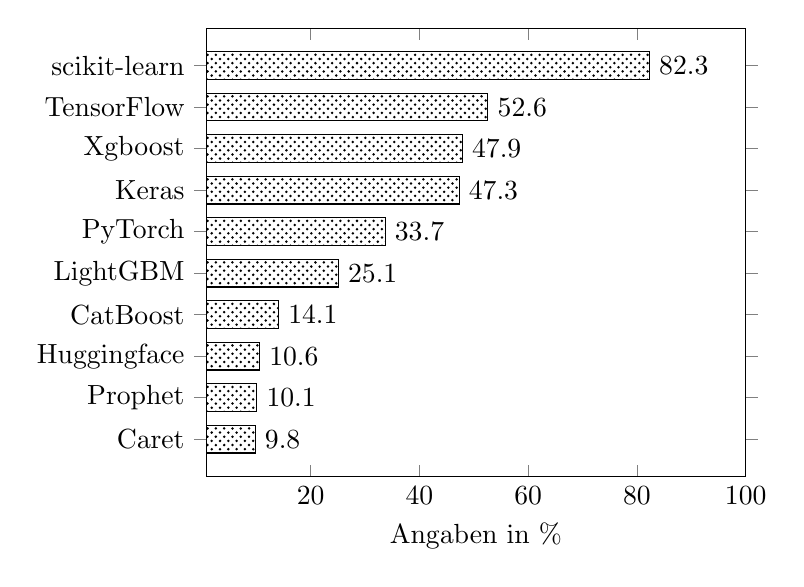
\begin{tikzpicture}
    \begin{axis}[
        xbar,
        xmax=100,
        nodes near coords,
        xlabel={Angaben in \%},
        symbolic y coords={Caret,Prophet,Huggingface,CatBoost,LightGBM,PyTorch,Keras,Xgboost,TensorFlow,scikit-learn},
        ytick = data,
  ]
  \addplot [pattern=crosshatch dots,pattern color=black] coordinates { (82.3,scikit-learn)(52.6,TensorFlow)(47.9,Xgboost)(47.3,Keras)(33.7,PyTorch)(25.1,LightGBM)(14.1,CatBoost)(10.6,Huggingface)(10.1,Prophet)(9.8,Caret)};
  \end{axis}
\end{tikzpicture}
\caption{Nutzung von ML-Frameworks \cite[]{kaggle}} \label{fig:kaggle}
\end{center}
\end{figure}

\noindent Aus der Grafik lassen sich drei der zu untersuchenden Python Bibliotheken entnehmen.
An erster Stelle steht \textit{scikit-learn}, das aufgrund der Vielzahl an implementierten Algorithmen wie ein \glqq Schweizer Taschenmesser\grqq{}
für die meisten Projekte eingesetzt werden kann und von über 80\% der Befragten verwendet wird.
Scikit-learn ist folglich bei der Auswahl der ML Bibliotheken unverzichtbar.
Die Vorteile von scikit-learn ist die benutzerfreundliche Struktur und Dokumentation mit der Machine Learning
auch für unerfahrene oder fachfremde Menschen zugänglich gemacht wird \cite[]{10.1145/2786984.2786995}.\\
\indent An zweiter Stelle steht \textit{TensorFlow}, das von über 50\% der Befragten benutzt wird und daher ebenfalls in
dem vorliegenden Ansatz untersucht wird.
Nachdem TensorFlow 2015 von Forschern bei Google ursprünglich für interne Zwecke entwickelt wurde, hat sich TensorFlow vor allem im Bereich
Deep Learning als populäres Werkzeug bewährt.
So bietet TensorFlow Projekte, die viel Customizing erfordern, eine leistungsfähige und flexible Umgebung, die das Trainieren
künstlicher neuronaler Netze vereinfacht und beschleunigt \cite[]{doi:10.3102/1076998619872761}.\\
\indent Die dritte zu untersuchende Bibliothek \textit{PyTorch} wird zwar insgesamt weniger häufig verwendet, verzeichnet
jedoch Jahr für Jahr ein starkes Wachstum in der Nutzung \cite[]{kaggle}.
PyTorch ist vor allem nützlich beim Umgang mit künstlichen neuronalen Netzen, weshalb es 2019 auch die
meistgenutzte Deep Learning-Bibliothek auf allen großen Deep Learning-Konferenzen war \cite[]{2020}.\\

\section{Web Scraping der ML-Klassen}\label{scrape}
Bevor im Source Code nach den Konfigurationsoptionen gesucht werden kann, ist es erforderlich, sich einen Überblick über
die zu untersuchenden Bibliotheken zu verschaffen.
Über die Dokumentation der Websites der Bibliotheken erhält man einen Einblick in die jeweilige Modul- und Klassenstruktur.
Da die gesuchten Optionen als Parameter von ML-Klassen übergeben werden, zielt dieser Ansatz darauf ab, alle Klassen
mitsamt der möglichen Parameter mit Hilfe von Web Scraping zu extrahieren.
Aufgrund des systematischen Aufbaus der verschiedenen Websites, kann man an dieser Stelle mit technischer Unterstützung
die gesuchten Daten automatisiert erfassen.
Die Python-Bibliothek \textit{Beautiful Soup} stellt für diesen Zweck, das notwendige Werkzeug bereit.
Beautiful Soup ist ein populäres Werkzeug für Web Scraping in Python.
So können strukturierte Daten aus HTML- oder XML-Dokumenten als Syntaxbaum geparst werden.
Mit einer Reihe verschiedener Methoden kann dieser dann analysiert oder die benötigten Informationen
extrahiert werden \cite[]{richardson2007beautiful}.\\

\noindent Der Scraping-Prozess lässt sich für die drei verschiedenen ML-Bibliotheken in folgende Schritte einteilen, die über die Klasse
\textit{ClassScraper} aufgerufen werden können.

\tikzstyle{form} = [rectangle, rounded corners, minimum height=1.67cm,text centered, text width=2.5cm, draw=black]
\tikzstyle{arrow} = [thick,->,>=stealth, text width=1.5cm, text centered]

\begin{center}
\begin{tikzpicture}[node distance=1.75cm]
\node (start) [form] {Modul-URLs scrapen};
\coordinate[left of=start] (d2);
\draw [arrow] (d2) -- node[anchor=east] {Doku-URL} (start);
\node (first) [form, right of=start, xshift=2cm] {Klassen-URLs scrapen};
\draw [arrow] (start) -- (first);
\node (second) [form, right of=first, xshift=2cm] {Klassen + Parameter scrapen};
\draw [arrow] (first) -- (second);
\coordinate[right of=second] (d1);
\draw [arrow] (second) -- node[anchor=west] { JSON-Datei} (d1);
\end{tikzpicture}
\end{center}
\

\noindent Je nach Komplexität der Dokumentation, werden diese Schritte teilweise in weitere kleinere Schritte unterteilt.
Zudem werden die Informationen in einem jeweils unterschiedlichen HTML-Format abgebildet,
sodass kein generischer Algorithmus über alle drei Dokumentationen laufen kann.
Deshalb wird für jede Bibliothek eine eigene Klasse implementiert, die vom ClassScraper zielführende Methoden erbt und
bei einer abweichenden Dokumentationsstruktur Methoden überschreibt. \\

\noindent Listing \ref{scrape_moduls} zeigt wie beispielsweise die Modul-URLs aus der Dokumentation von PyTorch extrahiert werden.
Um mit dem Scrapen der Daten zu beginnen, wird über über das \textit{request}-Modul der Python-Bibliothek \textit{urllib} die URL geöffnet.
Die HTML-Datei der URL wird in Beautiful Soup geparst, um auf die Daten der Seite zugreifen zu können.
In einem HTML-Dokument werden die Inhalte baumartig gespeichert.
Die Knoten dieses Baums werden mit sogenannten \textit{Tags} versehen, die dem Inhalt Form und Struktur verleihen.
Um auf den Bereich der Seite zuzugreifen, in dem die PyTorch-Module verlinkt sind, wird der Bereich über die Beautiful Soup-Methoden
\textit{find, find\_next} und \textit{findAll} weiter eingegrenzt.
Zunächst wird ein Paragraph (\textit{p}) vom Typ \textit{caption} gesucht, dessen Text \textit{Python API} ist.
Die einzelnen Modul-Links befinden sich in der nächstliegenden Liste, die mit dem Tag \textit{ul} (\textit{unordered list})
versehen ist.
Von dem Paragraph ausgehend, wird diese Liste mit der \textit{find\_next}-Methode erreicht.
Die Elemente der Liste sind mit einem \textit{li}-Tag (list item) versehen und werden extrahiert und als Set gespeichert.
Durch dieses Set wird iteriert, um für jedes Modul die Hyperlink-Referenz zu speichern.\\

\noindent\begin{minipage}{\linewidth}
\begin{lstlisting}[language=Python, frame=single, label=scrape_moduls, basicstyle=\small, caption={Web Scraping der Modul-URLs von PyTorch},captionpos=b]
def scrape_module_urls(self):
    link = "https://pytorch.org/docs/stable/index.html"
    html = urllib.urlopen(link)
    soup = bs4.BeautifulSoup(html, "html.parser")

    caption = soup.find("p", {"class": "caption"},
                        text="Python API")
    ul = caption.find_next("ul")
    li = ul.findAll("li", {"class": "toctree-l1"})

    for element in li:
        url = element.find("a").attrs["href"]
        self.module_urls.append(url)
\end{lstlisting}
\end{minipage}
\

\noindent Im Anschluss kann nun durch die Liste der Modul-URLs iteriert werden, um die Klassen zu extrahieren.
Die Hyperlinks der Module werden ebenfalls mit urllib geöffnet und die HTML-Datei in Beautiful Soup geparst.
Je nach Layout der Dokumentation werden mit Hilfe eben angesprochenen Beautiful Soup-Methoden schlussendlich alle
Klassen inklusive der Parameter gefunden und in einer JSON-Datei gespeichert werden.
In der JSON-Datei wird für jede Klasse der gesamte Pfad als eindeutiger Schlüssel angegeben.
Zusätzlich zum Klassen- und zu den Parameternamen, werden die Default-Werte der einzelnen Parameter aufgeführt.
Die scikit-learn-Klasse \textit{KNeighborsRegressor} wird demnach wie folgt gespeichert:\\

\noindent\begin{minipage}{\linewidth}
\begin{lstlisting}[frame=single, label=json_scraping, basicstyle=\small, caption={Web Scraping Ergebnis der KNeighborsRegressor-Klasse aus scikit-learn},captionpos=b]
"sklearn.neighbors.KNeighborsRegressor": {
    "short name": "KNeighborsRegressor",
    "parameters": {
        "n_neighbors": "5",
        "*": null,
        "weights": "'uniform'",
        "algorithm": "'auto'",
        "leaf_size": "30",
        "p": "2",
        "metric": "'minkowski'",
        "metric_params": "None",
        "n_jobs": "None"
    }
}
\end{lstlisting}
\end{minipage}
\

\noindent Im Gegensatz zu den anderen Modulen ist der Web Scraping Vorgang nur einmal je Bibliothek notwendig und muss nicht für jedes Projekt
von neuem gestartet werden.
Die am Ende erzeugte JSON-Datei bildet die Basis für das Extrahieren von Konfigurationsoptionen und kann für beliebige viele
Projekte verwendet werden.
Da bei diesem Vorgang eine Vielzahl an Websites angesteuert werden, handelt es sich hierbei um das Modul mit der längsten Laufzeit.
Das Skript ist allerdings anfällig gegenüber Änderungen im Layout der Website.
So können beispielsweise Änderungen der HTML-Elemente dazu führen, dass nicht mehr dieselben Ergebnisse erzielt werden. \\

\noindent Das Python-Skript kann sowohl über eine Entwicklungsumgebung, als auch über die Kommandozeile ausgeführt werden.
Um Python-Dateien über die Kommandozeile auszuführen, muss man lediglich den Befehl \textit{python3} oder bei älteren
Versionen \textit{python}, gefolgt vom Namen der Python-Datei eingeben.
Zusätzlich ist es möglich neben diesem Befehl noch weitere Werte hinzugefügt werden.
Diese sogenannten Argumente können im Source Code verarbeitet werden, um den Anwendenden eine Gestaltungsspielraum für
die Ausführung zu überlassen.
In diesem konkreten Fall wird über die Eingabe des Namens der Bibliothek entschieden, von welcher Bibliothek die
Klassen extrahiert werden sollen.
Damit auch bei unterschiedlichen Schreibweisen einer Bibliothek das Programm ausgeführt wird, sind im Source Code für jede
der drei Bibliotheken Tensorflow, PyTorch und scikit-learn mehrere Möglichkeiten hinterlegt.
Das Scraping von scikit-learn-Klassen erfolgt zum Beispiel über folgenden Befehl:\\

\noindent\begin{minipage}{\linewidth}
\begin{lstlisting}[language=bash, frame=single, label=scraping_scikit-learn, basicstyle=\small, caption={Kommandozeilenbefehl für das Web Scraping von scikit-learn},captionpos=b]
python3 scraping.py scikit-learn
\end{lstlisting}
\end{minipage}
\

\section{Parsen der Repositorys}
Der erste Schritt, um die Konfigurationsoptionen zu extrahieren, ist eine Umgebung zu schaffen, in der ein zu untersuchendes
Git-Repository vorliegt.
Über die \textit{GitPython}-Bibliothek wird das Repository geklont, sodass es lokal für die Analyse verfügbar ist.
Da sich die Analyse auf Source Code in Python bezieht, werden im nächsten Schritt alle Ordner sukzessiv nach Dateien mit
einer \textit{.py}-Endung durchsucht.
Diese Python-Dateien werden in einer Liste gespeichert, durch die in der Folge iteriert wird, um die Konfigurationsoptionen auszulesen. \\
\noindent Analog zum Web Scraping kann der gesamte Parse- und Extraktionsprozess inklusive der Datenflussanalyse über die Kommandozeile gestartet werden.
Die zu übergebenen Argumente sind zum Einen der Link des zu untersuchenden Git-Repositorys und zum Anderen die ML-Bibliothek, dessen
Konfigurationselemente gefunden werden sollen.
Der entsprechende Befehl für ein Beispielprojekt mit scikit-learn sieht demnach wie folgt aus: \\

\noindent\begin{minipage}{\linewidth}
\begin{lstlisting}[language=bash, frame=single, label=execute_coop, basicstyle=\small, caption={Kommandozeilenbefehl für die Extraktion von Konfigurationsoptionen von scikit-learn},captionpos=b]
python3 main.py https://github.com/user/project scikit-learn
\end{lstlisting}
\end{minipage}
\

\noindent Im Gegensatz zum Web Scraping erfolgt der gesamte Parse- und Extraktionsprozess für die zu untersuchenden Bibliotheken generisch.
Die Klasse \textit{ConfigOptions} enthält alle Methoden, um aus den Repositorys die Konfigurationsoptionen auszulesen.
Für jede der drei Bibliotheken gibt es eine Klasse, die von der \textit{ConfigOptions} abgeleitet ist und ihre Funktionen erbt.
Dadurch lässt sich dieses Tool beliebig auf andere Bibliotheken erweitern.
Voraussetzung ist jedoch, dass eine JSON-Datei mit den gescrapten Klassen der jeweiligen Bibliothek im entsprechendem Format vorliegt.
Möchte man beispielsweise die Funktionalitäten dieses Tools auf die ML-Bibliothek \textit{Keras} anwenden, muss man nach erfolgreichem Scraping,
lediglich folgende Codezeilen zur \textit{main.py}-Datei hinzufügen.\\

\noindent\begin{minipage}{\linewidth}
\begin{lstlisting}[language=Python, frame=single, label=keras,  basicstyle=\small, caption={Implementation einer Klasse zur Extraktion von Konfigurationsoptionen einer weiteren ML-Bibliothek},captionpos=b]
class KerasOptions(ConfigOptions):
    def __init__(self, repo):
        ConfigOptions.__init__(self, repo)
        self.library = "keras"
\end{lstlisting}
\end{minipage}
\

\section{Extraktion der ML-Klassen}\label{Classes}
Als nächstes werden die Klassen der jeweiligen ML-Bibliothek aus dem Source Code extrahiert.
Dafür wird durch die Liste mit Python-Dateien iteriert, der Source Code als AST geparst und entlang der AST Struktur
nach den entsprechenden Klassen gesucht.
Der Extraktion-Prozess der ML-Klassen lässt sich in vier Schritte einteilen, die über die Klasse
\textit{MLClasses} aufgerufen werden können.

\begin{enumerate}
 \item JSON-Datei mit gescrapten Klassen einlesen
 \item Code aus Python-Datei als AST parsen
 \item Traversierung des AST
\begin{enumerate}
    \item AST-Knoten nach Import-Anweisungen der ML-Bibliothek durchsuchen
    \item AST-Knoten, die Import-Bezeichnungen enthalten filtern
    \item Prüfen, ob es sich um ML-Klassen handelt
    \item ML-Klassen als Dictionary speichern
    \end{enumerate}
 \item Liste mit Dictionaries zurückgeben
\end{enumerate}

%\begin{center}
%\begin{tikzpicture}[node distance=1.75cm]
%\node (start) [form] {Code als AST parsen};
%\coordinate[left of=start, yshift=0.25cm] (d0);
%\coordinate[left of=start] (d1);
%\draw [arrow] (d0) -- node[anchor=east, yshift=0.25cm, text width=3cm] {JSON-Datei} (start);
%\draw [arrow] (d1) -- node[anchor=east, text width=3cm] {Python-Datei} (start);
%\node (first) [form, below of=start] {Klassen-URLs scrapen};
%\draw [arrow] (start) -- (first);
%\node (second) [form, below of=first] {Klassen + Parameter scrapen};
%\draw [arrow] (first) -- (second);
%\coordinate[right of=second] (d1);
%\draw [arrow] (second) -- node[anchor=west] { JSON-Datei} (d1);
%\end{tikzpicture}
%\end{center}
%\
\noindent Zunächst wird die JSON-Datei mit den gescrapten Klassen eingelesen und der Python-Code über die \textit{ast}-Bibliothek in das AST-Format umgewandelt.
Die Traversierung des Syntax-Baumes erfolgt nach dem Preoder-Verfahren, sodass jeder Knoten eines Teilbaums vollständig
durchlaufen wird, bevor der nächste Knoten auf der gleichen Stufe betrachtet wird.
Im ersten Schritt werden alle Import-Objekte rausgefiltert, um festzustellen, ob und wie die ML-Bibliothek verwendet wird.
Import-Objekte, die die ML-Bibliothek betreffen, werden in einer Liste gespeichert und bilden die Basis für die Suche nach
den ML-Klassen.
Es gibt verschiedene Möglichkeiten wie Elemente einer ML-Bibliothek zugänglich gemacht werden können.
Das folgende Codebeispiel zeigt fünf Möglichkeiten, die die Verwendung derselben scikit-learn-Klasse \textit{KNeighborsRegressor}
über einen jeweils anderen Pfad im Code ermöglichen. \\

\noindent\begin{minipage}{\linewidth}
\begin{lstlisting}[language=Python, frame=single, label=import,  basicstyle=\small, caption={Import- und Verwendungsmöglichkeiten der KNeighborsRegressor-Klasse aus scikit-learn},captionpos=b]
import sklearn                                           # A
import sklearn as skl                                    # B
from sklearn import neighbors                            # C
from sklearn.neighbors import KNeighborsRegressor        # D
from klearn.neighbors import KNeighborsRegressor as KNN  # E

sklearn.neighbors.KNeighborsRegressor()                  # A
skl.neighbors.KNeighborsRegressor()                      # B
neighbors.KNeighborsRegressor()                          # C
KNeighborsRegressor()                                    # D
KNN()                                                    # E
\end{lstlisting}
\end{minipage}
\

\noindent Die Eindeutigkeit des Pfades ist wichtig, um sicherzustellen, dass es sich bei dem jeweiligen Code-Objekt, um die Klasse
einer ML-Bibliothek handelt.
Einige Klassen haben geläufige Bezeichnungen, wie zum Beispiel \textit{Pipeline} aus scikit-learn.
Um zu vermeiden, dass irrtümlicherweise falsche Objekte gefunden werden, werden die Code-Objekte aus dem AST auf Basis der
Import-Anweisungen der jeweiligen ML-Bibliothek rausgefiltert.\\
\indent Angenommen das Codebeispiel in Listing \ref{knn} wird auf Klassen aus der scikit-learn-Bibliothek untersucht.\\

\noindent\begin{minipage}{\linewidth}
\begin{lstlisting}[language=Python, frame=single, label=knn,  basicstyle=\small, caption={Codebeispiel mit KNeighborsRegressor-Klasse},captionpos=b]
from sklearn.neighbors import KNeighborsRegressor

def knn_func():
    n_neighbors = 6
    knn = KNeighborsRegressor(n_neighbors, leaf_size=25)
    return knn
\end{lstlisting}
\end{minipage}
\

\noindent Für das Codebeispiel wird der Syntaxbaum nach Knoten durchsucht, deren Name identisch mit \textit{KNeighborsRegressor} ist und
vom AST-Typ \textit{Call} ist.
Der AST-Typ versichert, dass ein (Klassen-)Aufruf vorliegt und nicht beispielsweise ein gleichnamiger String ohne Klassenbezug.
Ist dies zutreffend, wird geprüft, ob es sich bei diesem Knoten um eine ML-Klasse handelt oder um einen Pfad, an dessen Ende eine ML-Klasse steht.
Ist auch dies gegeben, wird der gesamte Pfad des Objekts beleuchtet, um die Klasse eindeutig zuordnen zu können.
Dieser Schritt ist wichtig, da Klassenamen nicht immer eindeutig sind.
So verfügt beispielsweise PyTorch über zwei unterschiedliche \textit{profiler}-Klassen.
Die eine Klasse ist Teil des \textit{autograd}-Moduls, während die andere dem \textit{profiler}-Modul zugeordnet ist.
Beide verfügen über unterschiedliche Konfigurationsoptionen.
An dieser Stelle sollte man sich nicht irritieren lassen, dass die beiden Klassen kleingeschrieben sind.
Die Namenskonvention, dass Klassen mit Großbuchstaben beginnen, wird von den ML-Bibliotheken nicht immer eingehalten.\\
\indent Es kann auch der Fall eintreten, dass eine neu implementierte Klasse von einer ML-Klasse erbt.
So ist beispielsweise die PyTorch-Klasse \textit{Module} die Basisklasse für künstliche neuronale Netze \cite[]{NEURIPS2019_9015}.
Wenn Anwendende ein neuronales Netz implementieren wollen, rufen sie nicht die Module-Klasse nicht auf, sondern erben von ihr.
Um solche Fälle zu erfassen, wird beim Traversieren des Syntaxbaumes daher zusätzlich nach Klassendefinition (AST-Typ \textit{ClassDef}) gesucht und geprüft,
ob als Basisklasse eine ML-Klasse vorliegt. \\
\indent Die gefundene Klasse aus Listing \ref{knn} wird als Listenelement in Form eines Dictionaries gespeichert.
Das Dictionary enthält nun alle benötigten Informationen, um im nächsten Schritt
die Konfigurationsoptionen auszulesen.
Dazu gehört der vollständige Pfad mit dem Namen der Klasse, der verwendete Pfad inklusive Alias, sowie die Datei, indem
die Klasse gefunden wurde.
Zudem wird das AST-Objekt gespeichert, aus dem sich weitere Informationen wie Parameter und Zeilennummer auslesen lassen.
Für das Codebeispiel ergibt sich folgender Listeneintrag.\\

\noindent\begin{minipage}{\linewidth}
\begin{lstlisting}[frame=single, label=class_dict, basicstyle=\small, caption={Dictionary-Eintrag der KNeighborsRegressor-Klasse},captionpos=b]
{'class': 'sklearn.neighbors.KNeighborsRegressor',
 'class alias': 'KNeighborsRegressor',
 'file': 'path/file.py',
 'object': <ast.Assign object at 0x106178370>}
\end{lstlisting}
\end{minipage}
\

\section{Extraktion und Verarbeitung der Konfigurationsoptionen} \label{Parameters}
Der nächste Vorgang gliedert sich in zwei Teilschritte, bei dem die Ergebnisse aus \ref{scrape} und \ref{Classes} miteinander
verbunden werden.

\begin{enumerate}
 \item Extraktion der Parameterwerte aus AST-Objekt des Dictionaries
 \item Zuordnung der Werte zu den gescrapten Parametern aus JSON-Datei
\end{enumerate}

\noindent Zunächst wird durch die Liste mit Dictionaries aus \ref{Classes} iteriert.
Jedes Dictionary wird zusätzlich mit einem Eintrag zu den gescrapten Parametern der jeweiligen Klasse ergänzt und an die Methode \textit{get\_parameters()}
der Klasse \textit{MLParameters} übergeben.
In dieser Klasse wird der Syntaxbaum des Code-Objekts traversiert, um die übergebenen Parameterwerte in der
entsprechenden Reihenfolge zu extrahieren.
Die Klasse verfügt über eine Vielzahl an Methoden, die die einzelnen Knoten des Syntaxbaums entsprechend ihres Typs
verarbeiten können.
Da die gesuchten Werte Parameter von Klassenaufrufen sind, ist die Behandlung von Knoten des AST-Typs \textit{Call} von
besonderer Bedeutung.
Hinter dem AST-Objekt des Dictionaries aus \ref{Classes} verbirgt sich folgender Syntaxbaum: \\

\noindent\begin{minipage}{\linewidth}
\begin{lstlisting}[frame=single, label=class_dict, basicstyle=\small, caption={AST der KNeighborsRegressor-Klasse},captionpos=b]
Assign(
    targets=[
        Name(
            id='knn',
            ctx=Store())],
    value=Call(
        func=Name(
            id='KNeighborsRegressor',
            ctx=Load()),
        args=[
            Name(
                id='n_neighbors',
                ctx=Load())],
        keywords=[
            keyword(
                arg='leaf_size',
                value=Constant(
                    value=25))]))
\end{lstlisting}
\end{minipage}
\

\noindent Ein Code-Objekt vom AST-Typ \textit{Call} besteht aus 3 Teilknoten.
Der Knoten \textit{func} gibt den Namen Aufrufs an.
Ist an dieser Stelle die \textit{id} des Knoten identisch zur ML-Klasse, werden im nächsten Schritt die Parameter
extrahiert.
Diese liegen zweigeteilt vor:
Im Knoten \textit{args} befinden sich Argumente, die nach ihrer Position übergeben und zugeordnet werden.
Im Gegenzug werden im Knoten \textit{keywords} Argumente zusammen mit der Parameterbezeichnung übergeben, sodass direkt kenntlich
ist, um welchen Parameter es sich handelt. \\
\indent Im gegebenen Beispiel wird die Variable \textit{n\_neighbors} als Positionsargument vom AST-Typ \textit{Name} klassifiziert.
Für jeden übergebenen Parameter wird der AST-Typ vermerkt, um weitere Informationen für die Analyse von ML-Konfigurationsoptionen
bereitzustellen.
Wenn Parameter vom AST-Typ \textit{Name} oder \textit{Attribute} vorliegen, werden diese zusätzlich vermerkt, um wie
in Kapitel \ref{dataflow} beschrieben, mittels Datenflussanalyse mögliche Werte für die Variablen zu ermitteln.
Das Keyword-Argument für \textit{leaf\_size} kann hingegen direkt zugeordnet werden und ist auch konstant. \\
\indent Zusätzlich zur Ermittlung der Parameter wird in der \textit{MLParameters}-Klasse auch geprüft, ob die Instanziierung der Klasse
einer Variable zugewiesen wird.
Im gegebenen Beispiel wird die Instanz der Klasse (\textit{value}) von der Variablen \textit{knn} (\textit{target}) referenziert.
Darüber hinaus kann eine Zuweisung auch über andere Wege als Keyword-Argument erfolgen:
bei der Definition einer Klasse oder Funktion und beim Aufruf eines Objekts.\\
\indent Wie in Kapitel \ref{Classes} wird auch hier der Fall, dass von einer ML-Klasse geerbt wird, gesondert behandelt.
Da in diesem Fall keine Klasse aufgerufen wird, sondern auf der Basis einer ML-Klasse eine neue Klasse erstellt wird, werden die Parameter aus der
\textit{\_\_init\_\_}()-Methode entnommen.
Die \_\_init\_\_()-Methode kann aufgerufen werden, um Attribute einer Klasse zu initialisieren.
Über das Schlüsselwort \textit{self} können Werte den Attributen der Klassen zugewiesen werden.
Hierbei handelt es sich um die gesuchten Konfigurationsoptionen.
Das Listing \ref{nn_module} zeigt ein Codebeispiel indem die Klasse \textit{Model} definiert wird und
von der PyTorch-Klasse \textit{Module} erbt, um trainierbare Schichten (layers) für ein neuronales Netz zu erstellen.
In dem Beispiel handelt es sich bei dem Attribut \textit{self.conv1} um eine Schicht, der die PyTorch-Klasse \textit{Conv2d}
zugeordnet wird.
Demnach hat die Konfigurationoption \textit{conv1} den Wert \textit{nn.Conv2d(10, 20, 5)}.\\

\noindent\begin{minipage}{\linewidth}
\begin{lstlisting}[language=Python, frame=single, label=nn_module,  basicstyle=\small, caption={Vererbung der ML-Klasse Module aus PyTorch},captionpos=b]
import torch.nn as nn

class Model(nn.Module):
    def __init__(self):
        self.conv1 = nn.Conv2d(10, 20, 5)
\end{lstlisting}
\end{minipage}
\

\noindent Im zweiten Teil werden die gefundenen Parameter im Code mit den gescrapten aus der JSON-Datei zusammengeführt.
Zunächst wird durch die Liste an Positionsargumente iteriert, sodass die Positionsargumente der Reihe nach,
den gescrapten Parameter zugeordnet werden können.
Für die Keyword-Argumente wird geprüft, ob das Keyword als Parameter vorhanden ist.
Bei falschen Keyword-Bezeichnungen, also Keywords, die es als Parameter in der Spezifikation gar nicht gibt,
kann keine Zuordnung zu den gescrapten Parametern erfolgen. \\
\indent Darüber hinaus gibt es drei Besonderheiten in der Spezifikation, die vom Algorithmus bei der Zuordnung der Parameter
beachtet werden müssen: \textit{*}, \textit{*args} und \textit{**kwargs}.
Befindet sich in der Spezifikation der Parameter ein Sternchen, dürfen danach keine Positionsargumente mehr
übergeben werden.
Bei der Spezifikation der Parameter der \textit{KNeighborsRegressor}-Klasse aus Listing \ref{json_scraping} befindet 
sich dieses Sternchen an zweiter Stelle.
Dementsprechend müssen alle Parameter ab dem zweiten Parameter \textit{leaf\_size} als Keyword-Argumente übergeben werden.
\textit{*args} werden verwendet, wenn die Anzahl der Übergabeparameter variabel bleiben soll oder die Parameter in Form
eines Tupels oder einer Liste vorliegen.
Im ersten Fall kann die Länge der übergebenen Parameter, die Länge der Parameter in der Spezifikation also überschreiten.
Die \textit{überzähligen} Parameter werden zusammen mit dem letzten übergebenen Parameter als Tupel zusammengefasst.
Die Übergabe als Tupel oder als Liste erfolgt mit einem anführenden Sternchen.
\textit{**kwargs} hingegen sind eine Möglichkeit, um Dictionaries zu übergeben, die als Schlüssel Parameter der Klasse
enthalten können. \\

\noindent Nachdem die Parameter erfolgreich zugeordnet wurden, gibt die \textit{MLParameters}-Klasse ein Dictionary zurück.
Es enthält wie das Dictionary aus \ref{Classes} den Namen der Python-Datei, den vollständigen Pfad der Klasse und das AST-Objekt.
Ergänzt wird das Dictionary mit Informationen zu den Parametern.
Variable Parameter werden zusätzlich gesondert in einem Dictionary aufgeführt.
Da die möglichen Werte der variablen Parameter noch unbekannt sind, werden diese mit \textit{None} gekennzeichnet.
Sofern vorhanden, wird die Variable, die die Klasse referenziert, ebenfalls aufgeführt, sodass sich für das Codebeispiel
aus \ref{knn} folgendes Dictionary ergibt:\\

\noindent\begin{minipage}{\linewidth}
\begin{lstlisting}[frame=single, label=param_dict, basicstyle=\small, caption={Dictionary-Eintrag der KNeighborsRegressor-Klasse inklusive Parameter},captionpos=b]
{'class': 'sklearn.neighbors.KNeighborsRegressor',
 'file': 'path/file.py',
 'object': <ast.Assign object at 0x106178370>},
 'parameter': {'leaf_size': {'type': 'Constant',
                             'value': '25'},
               'n_neighbors': {'type': 'Name',
                               'value': 'n_neighbors'}},
 'variable': 'knn',
 'variable parameters': {'n_neighbors': None}}
\end{lstlisting}
\end{minipage}
\

\section{Ermittlung variabler Konfigurationswerte}\label{dataflow}
Zunächst wird durch die Liste mit Dictionaries aus Kapitel \ref{Parameters} iteriert.
Die Ermittlung der variablen Parameterwerte erfolgt über die \textit{get\_parameter\_value()}-Methode der \textit{DataFlowAnalysis}-Klasse.
Beim Aufruf der Methode wird für dieses Beispiel das Dictionary zusammen mit der Parametervariable \textit{n\_neighbors} übergeben.
Die anschließende Datenflussanalyse lässt sich in zwei Bereich einteilen:

\begin{enumerate}
 \item Sammeln von Informationen: Kontrollflüsse, Aufrufpfade und Funktionsaufrufe
 \item Analyse der Informationen mittels SSA, Constant Propagation und AST
\end{enumerate}

\noindent Im ersten Schritt wird über die \textit{CFGBuilder}-Klasse des statischen-Analyse-Frameworks \textit{Scalpel} der
Kontrollflussgraph für die Python Datei erstellt und in einer Liste gespeichert.
Der Kontrollflussgraph stellt alle globalen Pfade dar, die während der Ausführung des Programms durchlaufen werden können.
Da Klassen- und Funktionskörper sich jedoch nicht auf dieser Ebene befinden, wird zusätzlich jede Klasse und Funktion
der globalen Ebene traversiert und die Kontrollflussgraphen dieser Objekte ebenfalls in der Liste gespeichert.
Dieser Vorgang wiederholt sich für jede weitere Ebene bis schließlich alle Kontrollflussgraphen der
Klassen und Funktionen der Liste hinzugefügt wurden. \\
\indent Im nächsten Schritt werden die möglichen Pfade, mit denen man die einzelnen Klassen und Funktionen erreichen kann, ermittelt.
Diese Ermittlung ist erforderlich, da die Werte gesuchter Parametervariablen möglicherweise über Klassen und Funktionen hinweg
übergeben werden.
Der Aufrufspfad einer Funktion oder einer Klasse variiert jedoch je nachdem von wo sie aufgerufen werden.
Im folgenden sind vier Beispiele aufgelistet, die zeigen, dass es notwendig ist, die Objektzugehörigkeit und die damit
verbundenen Aufrufspfade zu kennen.

\begin{itemize}
 \item \textit{func()}: ruft globale Funktion auf
 \item \textit{self.func()}: Funktion befindet in einer Klasse und wird innerhalb dieser Klasse aufgerufen
 \item \textit{C.func()}: Funktion befindet sich in Klasse \textit{C} und wird von außerhalb der Klasse aufgerufen
 \item \textit{C(1)}: ruft die \textit{\_\_init\_\_}-Methode der Klasse \textit{C} auf
\end{itemize}

\noindent Für jede Klasse und jede Funktion wird daher ein Dictionary erstellt, dessen Werte die möglichen Aufrufpfade sind.
Ohne Kenntnisse der Aufrufpfade würde ansonsten bei der Datenflussanalyse beispielsweise der übergebene Wert im vierten Fall
nicht der richtigen Methode zugeordnet werden können.\\
\indent Im Anschluss wird durch die Liste der Kontrollflussgraphen iteriert und alle enthaltenen Anweisungen als AST geparst.
Der abstrakte Syntaxbaum wird traversiert, um Funktionsaufrufe rauszufiltern und in einer Liste zu speichern.
Nachdem alle Kontrollflussgraphen durchlaufen wurden, enthält die Liste sämtliche Funktionsaufrufe der Datei im AST-Format.
Falls nun die gesuchte Variable als Parameter in der Definition einer Funktion steht, können auf Basis der möglichen Pfade
der Funktion, die Funktionsaufrufe gefunden werden.
Dadurch kann der Wert einer Variable bzw. des Parameters über den gesamten Kontrollfluss der Datei verfolgt werden.\\

\noindent Nachdem im ersten Teil die notwendigen Informationen gesammelt wurden, werden diese im zweiten analysiert.
Für jeden Kontrollflussgraphen der Datei werden über die \textit{compute\_SSA()}-Methode der Scalpel-Klasse \textit{SSA} Zuweisungen
und Werte der enthaltenen Variablen ermittelt.
Dafür werden von der Methode die Datenflussanalyse-Techniken \textit{Static Single Assignment} und \textit{Constant Propagation}
verwendet.
Als Ergebnis erhält man eine Liste an Dictionaries.
Die Schlüssel sind Variablen, die Ziel einer Zuweisung sind, während die Werte des Dictionaries, den jeweiligen Wert der Zuweisung
entsprechen.
Wird der gesuchten Variable ein Wert zugewiesen, wird dieser in der Liste möglicher Werte gespeichert.
Handelt es sich zudem um einen variablen Wert vom AST-Typ \textit{Name} oder \textit{Attribute}, wird im Anschluss auch für diesen Wert
der gesamte zweite Teil der Datenflussanalyse ausgeführt.\\
\indent In diesem Zusammenhang stößt man an mehrere Grenzen des Scalpel-Frameworks, die im folgenden Codebeispiel dargestellt werden:\\

\noindent\begin{minipage}{\linewidth}
\begin{lstlisting}[language=Python, frame=single, basicstyle=\small, label=scalpel_limits, caption={Limitierungen der Datenflussanalyse},captionpos=b]
class A:
    def __init__(self):
        a, b = 1, 2                         # issue 1
        c = 3                               # issue 2
        self.cls_variable = c               # issue 3
        c = 4
\end{lstlisting}
\end{minipage}
\

\noindent Die aktuelle Scalpel-Version (vom 02.06.22) kann keine Zuweisungen an Tupel verarbeiten, sodass für die Variablen \textit{a} und \textit{b}
von derzeit keine Wertzuweisungen ausgegeben werden (\textit{issue 1}).
Zudem wird in der aktuellen Version nur die letzte Zuweisung.
Für die Variable \textit{c} beträgt der Wert bei der Ausgabe demnach \textit{4}, obwohl der Variable vorher ein anderer
Wert zugewiesen wird (\textit{issue 2}).
Das größte Problem ist jedoch, dass in der aktuellen Version von Scalpel Zuweisungen an Objekte des AST-Typs \textit{Attribute} nicht verarbeitet werden
und der Wert für \textit{self.cls\_variable} nicht ermitteln werden kann (\textit{issue 3}).
Da die Lösung dieses Problems essenziell für die Datenflussanalyse ist, wurde der Source Code der \textit{compute\_SSA()}-Methode
untersucht und so angepasst, dass nun auch Zuweisungen an Instanzvariablen wie \textit{self.cls\_variables} verarbeitet werden können.
Leider beträgt der Wert für \textit{c} wie in \textit{issue 2} beschrieben zum Zeitpunkt der Zuweisung der SSA-Analyse von Scalpel \textit{4}, obwohl
\textit{3} richtig ist.
Für diese Probleme wurden jeweils ein Issue, teilweise mit Lösungsansatz, im Git-Repository von Scalpel erstellt.
Zum Zeitpunkt der Fertigstellung dieser Arbeit wurden diese Probleme zwar zur Kenntnis genommen, jedoch noch nicht behoben.\\

\noindent Im nächsten Schritt werden die Funktionsdefinitionen der Datei untersucht, um zu überprüfen, ob die gesuchte Variable als
Parameter übergeben wird.
Ist die gesuchte Variable in der Definition der Funktion vorhanden, müssen einige Besonderheiten bei der Behandlung der Argumente
berücksichtigt werden.
Die Parameter einer Funktion können fünf unterschiedliche AST-Typen besitzen: \textit{arg}, \textit{vararg}, \textit{kwonlyargs},
\textit{posonlyarg} oder \textit{kwarg}.
Ähnlich wie die Argumente des Typs \textit{ast.Call} aus Kapitel \ref{Parameters} müssen die AST-Typen unterschiedlich behandelt werden, damit die Parametervariable
beim Aufruf der Funktion eindeutig zugeordnet werden kann.
Im folgenden Codebeispiel werden die verschiedenen Typen mit ihrem Namen kenntlich gemacht: \\

\noindent\begin{minipage}{\linewidth}
\begin{lstlisting}[language=Python, frame=single, basicstyle=\small, label=args, caption={Parametertypen von Funktionen},captionpos=b]
def func(posonlyarg1, posonlyarg2, /, arg1, arg2,
         arg3 = 1, *vararg, kwonlyarg1, kwonlyarg2, **kwarg):
    return

func("posonlyarg1", "posonlyarg2", arg2=2, *["arg1"],
     kwonlyarg1=1, kwonlyarg2=2, **{"arg3": 3, "new_arg": 0})
\end{lstlisting}
\end{minipage}
\

\noindent \textit{Positional-only arguments} sind Argumente, die vor der \textit{/}-Markierung stehen und dürfen nicht mit einem
Keyword-Argument übergeben werden.
Das Gegenstück dazu sind \textit{Keyword-only arguments}.
Sie müssen mit einem Keyword übergeben werden und befinden sich in der Definition immer nach \textit{varargs}.
\textit{Args} sind Argumente bei denen nicht festgelegt ist, ob sie mit einem Keyword übergeben werden.
Sie werden ansonsten ihrer Position nach zugeordnet.
Die Typen \textit{vararg} und \textit{kwarg} referenzieren die übergebenen \textit{*args}- und \textit{**kwargs}-Parameter,
die in Kapitel \ref{Parameters} besprochen wurden.
Ist die gesuchte Variable in der Definition der Signatur vorhanden, besteht die Möglichkeit, dass ihr wie bei \textit{arg3} ein Default-Wert
zugewiesen wird, der dementsprechend zur Liste möglicher Werte der Parametervariablen hinzugefügt werden muss \cite[]{9425916}.\\
\indent Im letzten Schritt der Datenflussanalyse wird, sofern die gesuchte Variable ein Funktionsparameter ist,
durch die Liste mit Funktionsaufrufen iteriert.
Jeder Funktionsaufruf wird mit den möglichen Werten aus der Liste an Dictionaries mit möglichen Aufrufspfaden verglichen und
einer Funktion zugeordnet.
Für jeden Aufruf der Funktion wird je nach Argumenttyp und Position der gesuchten Parametervariable, der übergebene
Wert ausgelesen.
Handelt es sich bei einem übergebenen Wert erneut um eine Variable, wird im Anschluss auch für diesen Wert
der gesamte zweite Teil der Datenflussanalyse wiederholt. \\

Nach erfolgreichem Durchlauf gibt die \textit{get\_parameter\_value()}-Methode der \textit{DataFlowAnalysis}-Klasse
eine Liste mit möglichen Werten zurück.
Die Liste wird im Anschluss in ein Dictionary umgewandelt, dessen Schlüssel aufsteigende Zahlen sind.
Schlussendlich wird eine JSON-Datei erstellt, die alle gesuchten Konfigurationsoptionen des Git-Repositories enthält.
Für das \textit{KNeighborsRegressor}-Beispiel sieht der Eintrag wie folgt aus: \\

\noindent\begin{minipage}{\linewidth}
\begin{lstlisting}[frame=single, label=final_dict, basicstyle=\small, caption={Dictionary-Eintrag der KNeighborsRegressor-Klasse mit möglichen Parameterwerten},captionpos=b]
{'file': 'path/file.py',
 'class': 'sklearn.neighbors.KNeighborsRegressor',
 'parameter': {'leaf_size': {'type': 'Constant',
                             'value': '25'},
               'n_neighbors': {'type': 'Name',
                               'value': 'n_neighbors'}},
 'variable parameters': {'n_neighbors': {'type': 'Constant',
                                         'value': '26'},
 'variable': 'knn',
 'line no': '4'}
\end{lstlisting}
\end{minipage}
\


\chapter{Evaluation}\label{Evaluation}
Im folgenden Kapitel werden die Ergebnisse aus Kapitel \ref{Methodik} evaluiert.
Zunächst werden die Resultate des Web Scraping-Moduls beleuchtet bevor im Anschluss der vorgestellte Ansatz
als Ganzes evaluiert wird.
Die Verwendung von Konfigurationsoptionen von ML-Bibliotheken im Source Code ist jedoch nicht umfassend erforscht,
weshalb es keine Datensätze oder Vergleichswerte gibt, um die Genauigkeit beurteilen zu können.
Dementsprechend wird der Ansatz auf zwei verschiedene Arten überprüft:
\begin{enumerate}
 \item Tests
 \item Analyse von Projekten
\end{enumerate}

\noindent Tests sind ein gängiges Mittel in der Softwareentwicklung.
Sie dienen der Qualitätssicherung, um die Funktionalität des Systems zu gewährleisten und zu untersuchen inwieweit
die gestellten Anforderungen an eine Software auch erfüllt werden.
In der \textit{tests.py}-Datei des Git-Repositorys zu dieser Arbeit befinden sich mehrere Codebeispiele mit Konfigurationsoptionen, die aus
verschiedenen Softwareprojekten entnommen wurden \cite[]{marco}.
Zudem werden auch weitere ausgedachte Codebeispiele getestet, um zu prüfen, ob der entwickelte
Ansatz auch komplexere Herausforderungen bewältigen kann.
Ziel des ganzen ist zu prüfen, ob die verwendeten ML-Klassen inklusive der Parameter richtig erkannt und zugeordnet werden.
Zudem wird getestet, ob die Werte variabler Parameter, die teilweise auch über Klassen und Funktionen hinweg weitergegeben werden,
bestimmt werden können.
Mit Hilfe des \textit{pytest}-Frameworks werden die gefundenen Konfigurationsoptionen des entwickelten Ansatzes,
mit dem tatsächlichen Ergebnis verglichen.
Falls sich die Ergebnisse unterscheiden, gibt pytest eine Fehlermeldung aus.\\
\indent Um darüber hinaus eine aussagekräftige Bewertung abzugeben, wird sich am Evaluationsansatz von \citeauthor{10.1145/1985793.1985812}
orientiert.
Dafür werden verschiedene Softwareprojekte mit dem vorgestellten Ansatz analysiert und das Ergebnis mit einer manuellen Analyse verglichen.
Für die manuelle Analyse wird der Source Code auf die Verwendung von Konfigurationsoptionen der zu untersuchenden ML-Bibliothek
händisch untersucht.\\

\section{Ergebnisse Web Scraping}
\begin{table}[H]
\small
\begin{center}
\begin{tabular}[h]{c|c|c|c|c|c}
\hline
ML-Bibliothek & Version & Laufzeit (min) & Klassen & Parameter & P/K\\
\hline \hline
TensorFlow & 2.9.1 & 27:15 & 844 & 3728 & 4,4\\
PyTorch & 1.11.0 & 0:37 & 408 & 1340 & 3,3 \\
scikit-learn & 1.1.1 & 0:31 & 262 & 2081 & 7,9\\
\hline
\end{tabular}
\caption{Scraping Ergebnisse der ML-Dokumentation} \label{scrapresults}
\end{center}
\end{table}

In der Tabelle \ref{scrapresults} wird für jede ML-Bibliothek die Anzahl an Klassen und Parameter, sowie die durchschnittliche
Anzahl der Parameter je Klasse (P/K) für die jeweilige Version dargestellt.
Zudem wird die Laufzeit des Web-Scraping-Vorgangs gemessen.
Die angegebene Zeit ist der Mittelwert aus fünf Durchläufen der Anwendung und kann je nach Internetverbindung und Rechnerleistung
stark variieren.
Die angegebenen Zeiten wurden mit einer LAN-Verbindung des Universitätsnetzwerks in Leipzig und
einem MacBook Pro mit M1 Pro Chip, 10-Core CPU und 16 Gigabyte Arbeitsspeicher erzielt.
Die Anzahl der Klassen steht dabei in Relation zur Dauer des Scraping-Prozesses.
Während das Web Scraping der Klassen aus der scikit-learn-Dokumentation die geringste Laufzeit hatte,
dauerte der Prozess bei TensorFlow deutlich am längsten an.
Weitere Einflussfaktoren auf die Laufzeit sind zudem die Dokumentations- und Modulstruktur.
Während in TensorFlow und scikit-learn für jede Klasse eine neue Website aufgerufen werden muss, um die Parameter zu extrahieren,
sind bei PyTorch teilweise mehrere Klassen inklusive der Parameter auf einer Seite aufgelistet.
TensorFlow und PyTorch weisen zudem eine hohe Zahl an Modulen auf und oft müssen mehrere Module durchlaufen werden, um zu einer Klasse zu gelangen.
Sciki-learn hingegen verfügt über eine eher flache Modultiefe, sodass die Klassen meist über einen kürzeren Pfad erreicht werden können.
Des Weiteren weisen die Klassen von scikit-learn im Schnitt eine deutlich höhere Zahl an Parametern und somit mehr Konfigurationsmöglichkeiten auf.\\
\indent Zu beachten ist, dass Erfolg und Reproduzierbarkeit des Scraping-Moduls stark mit der Website-Struktur der Dokumentation zusammenhängen,
da das Modul nicht Robust gegenüber Änderungen ist.
Ändert sich das Layout indem beispielsweise HTML-Elemente anders strukturiert werden, so kann es sein, dass der Scraping-Algorithmus nicht mehr die
gewünschten Ergebnisse liefert.
Gleichzeitig müssen insgesamt drei TensorFlow- und sechs PyTorch-Klassen einzeln zum Scraping-Ergebnis hinzugefügt werden,
da sie nicht wie die anderen Klassen in die Dokumentation eingebettet und mit den gleichen HTML-Tags versehen sind.\\

\section{Auswahl Subject Systems}
Die Auswahl der zu untersuchenden Softwaresysteme erfolgt nach folgenden Kriterien:
\begin{itemize}
 \item Open Source Git Repository mit mindestens 1.000 Sternen
 \item Verwendung von mindestens zehn Klassen einer ML-Bibliothek
 \item möglichst Verwendung von variablen Parametern beim Aufruf der Klassen
 \item Code ist syntaktisch fehlerfrei
\end{itemize}

\noindent Ein vergebener Stern für ein Git-Repository kann sowohl als Lesezeichen als auch als Zeichen der Wertschätzung für das Projekt dienen.
Aus der Anzahl an Sternen lassen sich somit Aussagen über die Popularität eines Projektes ableiten.
Daher eignet sich die Anzahl der Sterne als Auswahlkriterium für die Erstellung einer repräsentativen Liste an Softwareprojekten, die die
ML-Bibliotheken benutzen.
Um bei der Analyse auch möglichst viele verschiedene Fälle von ML-Konfigurationsoptionen abzudecken, müssen mindestens zehn
Klassen einer ML-Bibliothek verwendet werden.
Im besten Fall werden den ML-Klassen auch variable Parameter übergeben, um die Genauigkeit des Datenflussanalyse-Moduls
untersuchen zu können.
Damit der Code als AST geparst werden kann, muss er zudem syntaktisch fehlerfrei sein.\\
\indent Für jede der drei ML-Bibliotheken werden jeweils fünf Softwareprojekte untersucht, die in der Tabelle \ref{projekte} aufgelistet
werden.\\

\begin{table}[H]
\small
\begin{center}
\begin{tabular}[h]{l|l|c|c}
\hline
Projekt & ML-Bibliothek & letzter Commit & Sterne \\
\hline \hline
DeepSpeech & \multirow{5}{*}{TensorFlow} & 17.11.21 & 19.7k\\
Fast Style Transfer & & 18.09.21 & 10.5k \\
Darkflow & & 25.02.20 & 6k \\
Text Classification & & 21.07.18 & 5.5k \\
Tensorforce & & 10.02.22 & 3.1k \\
\hline
Voice Cloning & \multirow{5}{*}{PyTorch} & 01.03.22 & 35k\\
YOLOv3 & & 04.04.22 & 6.7k \\
Image Captioning & & 03.06.20 & 2k \\
BatchNorm & & 08.04.21 & 1.4k \\
TorchIO & & 25.05.22 & 1.4k \\
\hline
AutoGluon & \multirow{5}{*}{scikit-learn} & 03.06.22 & 4.5k\\
igel & & 06.02.22 & 3k \\
MLJAR & & 14.04.22 & 1.9k \\
KServe & & 03.06.22 & 1.5k \\
sklearn-porter & & 23.05.22 & 1.2k \\
\hline
\end{tabular}
\caption{Untersuchte Softwareprojekte} \label{projekte}
\end{center}
\end{table}

\noindent \textit{Tensorforce} ist ein \textit{Deep Reinforcement Learning}-Framework, dass auf Googles TensorFlow beruht \cite[]{tensorforce}.
\textit{CNN for Text Classification} und \textit{Fast Style Transfer} basieren ebenfalls auf TensorFlow und verwenden
sich faltende künstliche neuronale Netzwerke (\textit{Convolutional Neural Networks}) zur Textklassifizierung \cite[]{CNN_for_Text_Classification} und für eine
schnelle Stilübertragung von berühmten Gemälden auf beliebige Fotos \cite[]{Fast_Style_Transfer}.
Mit \textit{DeepSpeech} von Mozilla lässt sich Sprache zu Text auf einem Raspberry Pi verarbeiten \cite[]{DeepSpeech} und mit
\textit{Darkflow} Objekte in Echtzeit erkennen und klassifizieren \cite[]{Darkflow}.\\
\indent Bei \textit{Real-Time Voice Cloning} handelt es sich um ein Deep Learning Framework und ist das erste von fünf
analysierten PyTorch-Projekten \cite[]{Charles2013}.
In \textit{YOLOv3} ist der YOLO-Algorithmus zur Bilderkennung in Echtzeit implementiert \cite[]{YOLO_v3}.
\textit{PyTorch Tutorial to Image Captioning} ist eine Anleitung zur Bildbeschriftung \cite[]{a_PyTorch_Tutorial_to_Image_Captioning}.
\textit{TorchIO} bietet eine Reihe von Deep Learning Werkzeugen zur medizinischen Bildgebung \cite[]{perez-garcia_torchio_2021}
und \textit{Synchronized Batch Normalization} befasst sich mit synchronisierter Batch Normalisierung zur
Objekterkennung in PyTorch \cite[]{Synchronized_Batchnorm}.\\
\indent \textit{AutoGluon} verwendet scikit-learn und automatisiert ML-Aufgaben, um ML-Anwendungen mit geringerem
Aufwand entwickeln zu können \cite[]{agtabular}.
\textit{Igel} ist ein ML-Tool mit dem Modelle trainiert und verwendet werden können, ohne Code schreiben zu müssen \cite[]{igel}.
Bei \textit{MLJAR} handelt es sich um ein Python-Paket für \textit{AutoML} auf tabellarische Daten \cite[]{mljar}.
\textit{KServe} stellt eine benutzerdefinierte Ressourcendefinition für ML-Modelle beliebiger Frameworks
auf \textit{Kubernetes} bereit \cite[]{KServe}.
Mit \textit{sklearn-porter} können Schätzer von scikit-learn in andere Programmiersprachen übersetzt werden \cite[]{sklearn_porter}.

\section{Analyse Subject Systems}
Für die Evaluation wird für jedes der 15 Softwareprojekte auf das Auftreten von Konfigurationsoptionen der enthaltenen ML-Bibiliothek
einmal manuell und mit dem vorgestellten Ansatz untersucht.
Das Ergebnis beider Analysen wird am Ende verglichen, um die Genauigkeit des entwickelten Ansatzes beurteilen zu können.\\
\indent Im Rahmen der manuellen Analyse wird in jeder Python-Datei des Softwareprojekts untersucht, ob und welche Elemente der ML-Bibliothek
importiert werden.
Werden Elemente der ML-Bibliothek importiert, wird in der jeweiligen Python-Datei nach ihnen gesucht.
Bei jedem gefundenen Objekt wird geprüft, ob es sich um eine Klasse handelt.
Dies erfolgt durch einen Abgleich der Beschreibung des Objekts in der Dokumentation oder
über die Definition des Objekts im Source Code der ML-Bibliothek.
Die gefundenen Klassen werden inklusive der Parameter in einer separaten Textdatei gespeichert.
Werden variable Parameter übergeben, wird in der Python-Datei zusätzlich nach möglichen Wertzuweisungen für die Variablen gesucht.
Bei der Suche wird berücksichtigt, dass die Variablen auch über Aufrufe von Klassen und Funktionen übergeben werden können oder ihnen ebenfalls ein
variabler Wert zugewiesen werden kann.
Für diese Fälle werden die übergebenen Werte der jeweiligen Aufrufe betrachtet oder nach Zuweisungen für die neue Variable gesucht.
Die gefundenen Zuweisungen werden ebenfalls in separaten Textdatei gespeichert.\\
\indent Die Ergebnisse werden in der Tabelle \ref{manuell} zusammengefasst.
Für jedes der fünfzehn Softwareprojekte ist die Anzahl der gefundenen Klassen und Anzahl der
(variablen) Parameter angegeben.
Darüber hinaus werden für die variablen Parameter in der letzten Spalte die Anzahl der möglichen Werte anhand
der Wertezuweisungen aufgeführt.
An dieser Stelle sollte man sich nicht irritieren lassen, dass, wie bei Fast Style Transfer, die Anzahl der variablen Parameter
die Anzahl der Wertzuweisungen übersteigt.
Dies liegt daran, dass viele variable Konfigurationswerte bei der Initialisierung von Klassen oder Aufruf von Funktionen
übergeben werden.
Diese Aufrufe liegen jedoch nicht immer in derselben Python-Datei oder werden teilweise erst zur Laufzeit ermittelt.
Sie sind daher für die Datenflussanalyse in diesem Ansatz außerhalb des Betrachtungsrahmens.

\begin{table}[H]
\small
\begin{center}
\setlength{\tabcolsep}{5pt}
\begin{tabular}[h]{l|c|c|c|c} %p{7cm}
\hline
\multirow{2}{*}{ML-Projekt} & \multirow{2}{*}{Klassen}   & \multirow{2}{*}{Parameter} &   \multicolumn{2}{c}{variable Parameter}\\
                            &           &           &   insgesamt   &   Zuweisungen \\
\hline \hline
DeepSpeech                  & 34        & 48        & 24            & 31\\
Fast Style Transfer         & 18        & 10        & 4             & 3\\
Darkflow                    & 15        & 10        & 7             & 9\\
Text Classification         & 21        & 30        & 11            & 4\\
Tensorforce                 & 61        & 105       & 58            & 96\\
\hline
Voice Cloning               & 107       & 165       & 100           & 99\\
YOLOv3                      & 31        & 44        & 28            & 35\\
Image Captioning            & 32        & 49        & 34            & 26\\
BatchNorm                   & 14        & 21        & 4             & 3\\
TorchIO                     & 30        & 38        & 36            & 31\\
\hline
AutoGluon                   & 79        & 98        & 52            & 31\\
igel                        & 12        & 8         & 34            & 26\\
MLJAR                       & 33        & 110       & 22            & 29\\
KServe                      & 21        & 21        & -             & -\\
sklearn-porter              & 34        & 34        & 23            & 123\\
\hline
\end{tabular}
\caption{Ergebnis der manuellen Analyse} \label{manuell}
\end{center}
\end{table}

\noindent Im zweiten Schritt wird der entwickelte Ansatz auf die fünfzehn Softwareprojekte angewendet.
Dies erfolgt indem in der Kommandozeile der Befehl aus Listing \ref{execute_coop} angepasst für das jeweilige Repository und die
jeweilige ML-Bibliothek ausgeführt wird.
Zuvor wurden bereits über den Kommandozeilenbefehl aus Listing \ref{scraping_scikit-learn} die Klassen und Parameter
der ML-Bibliotheken aus den Dokumentationen extrahiert.
Die im Ausgabeergebnis erzeugte JSON-Datei wird mit den gefundenen Klassen, Parametern und Zuweisungen der manuellen
Analyse verglichen.
Für jedes gefundene Objekt der manuellen Analyse wird geprüft, ob es auch vom entwickelten Ansatz gefunden wird und
das Ergebnis in der Tabelle \ref{analyse} zusammengefasst.
Die Tabelle folgt demselben Schema wie die Tabelle \ref{manuell}.
Sie gibt jedoch eine Prozentzahl an, die die Genauigkeit des entwickelten Ansatzes misst.
Die Prozentzahl berechnet sich dabei aus dem Anteil der gefundenen Objekte im Vergleich zur manuellen Analyse.

\begin{table}[H]
\small
\begin{center}
\setlength{\tabcolsep}{5pt}
\begin{tabular}[h]{l|c|c|c|c} %p{7cm}
\hline
\multirow{2}{*}{ML-Projekt} & \multirow{2}{*}{Klassen}   & \multirow{2}{*}{Parameter} &   \multicolumn{2}{c}{variable Parameter}\\
                            &           &           &   insgesamt   &   Zuweisungen \\
\hline \hline
DeepSpeech                          & 100\%                     & 98\%                         & 100\%             & 100\%\\
Fast Style Transfer                 & 100\%                     & 100\%                         & 100\%             & 100\%\\
Darkflow                            & 100\%                     & 100\%                         & 100\%              & 100\%\\
Text Classification                 & 100\%                     & 100\%                        & 100\%              & 100\%\\
Tensorforce                         & 100\%                    & 100\%                         & 100\%             & 79\%\\
\hline
Voice Cloning                      & 100\%                    & 100\%                        & 100\%            & 97\%\\
YOLOv3                              & 100\%                    & 100\%                        & 100\%             & 100\%\\
Image Captioning                    & 100\%                    & 100\%                        & 100\%             & 96\%\\
BatchNorm                           & 100\%                     & 100\%                        & 100\%              & 100\%\\
TorchIO                             & 100\%                     & 100\%                       & 100\%             & 100\%\\
\hline
AutoGluon                           & 100\%                     & 100\%                       & 100\%            & 100\%\\
igel                              & 100\%                      & 100\%                        & 100\%             & 100\%\\
MLJAR                              & 100\%                   & 100\%                         & 100\%             & 93\%\\
KServe                            & 100\%                     & 100\%                         & -                  & -\\
sklearn-porter                      & 100\%                   & 100\%                         & 100\%            & 100\%\\
\hline
\end{tabular}
\caption{Ergebnis des entwickelten Ansatzes mit Prozentangabe für den Anteil der gefundenen Objekte gegenüber der manuellen Analyse} \label{analyse}
\end{center}
\end{table}

\noindent Der Vergleich der beiden Analysen ergibt, dass der Algorithmus alle Klassen und fast alle Parameter erkennen kann.
Schwächen hat das Programm lediglich bei der Erkennung von Zuweisungen.
Dies hat zwei Ursachen, die in Listing \ref{scalpel_limits} dargestellt sind:
Die aktuelle Version von Scalpel (vom 02.06.22) kann im Rahmen des \textit{Static Single Assignment} Zuweisungen an Tupel
nicht verarbeiten (\textit{issue 1}).
Bei Tensorforce ist dies elf- und bei Real-Time Voice Cloning einmal der Fall.
Die zweite Ursache ist die Verarbeitung mehrerer Zuweisungen an die gleiche Variable innerhalb eines Funktionskörpers (\textit{issue 2}).
Scalpel gibt aktuell nur den letzten Zuweisungswert als möglichen Wert der Variable aus.
Die vorherigen Zuweisungen des Funktionskörpers werden nicht ausgegeben.
Neun weitere Zuweisungen von Tensorforce, zwei von Real-Time Voice Cloning, zwei von MLJAR und
eine Zuweisung vom PyTorch Tutorial to Image Captioning werden dadurch nicht erkannt.
Die beiden Probleme wurden bereits den Entwicklern gemeldet und werden derzeit bearbeitet.
Darüber hinaus wird in DeepSpeech einer Instanz der TensorFlow-Klasse \textit{SparseTensor} erzeugt und der Parameter \textit{*transcript} übergeben.
Dass als Übergabeparameter eine Liste als \textit{*args} übergeben werden darf, ist aus der Dokumentation nicht ersichtlich
und wurde vom entwickelten Ansatz daher nicht erkannt und verarbeitet.\\

\section{Diskussion}
Die Analyse der Softwareprojekte zeigt, dass der entwickelte Ansatz die Verwendung von ML-Klassen und Parameter
mit einer sehr hohen Genauigkeit erkennt.
Die Kombination aus den extrahierten Daten aus den Dokumentationen der ML-Bibliotheken und der Verarbeitung des Source Codes als AST
harmonieren sehr gut, um die verwendeten Konfigurationsoptionen zu identifizieren.\\
\indent Hinsichtlich der Wertebestimmung variabler Parameter werden ebenfalls viele verschiedene Fälle abdeckt.
Gleichwohl unterliegt diese Wertebestimmung einigen Limitierungen, die auch das Ergebnis der manuellen Analyse beeinträchtigen.
Es gibt jedoch Möglichkeiten den Algorithmus zu verbessern, an denen teilweise, wie beim
Analyse-Frameworks Scalpel, bereits gearbeitet wird.
So werden nur Zuweisungen betrachtet, weshalb die Zahl möglicher Werte der Variablen deutlich höher sein kann.
Jede weitere Operation, die auf eine Variable angewendet wird, wird in diesem Ansatz nicht weiter erfasst.
Verbirgt sich hinter der Variable zum Beispiel eine Liste oder ein Dictionary, so wird nur der Wert der Variablen bei der
Initialisierung bestimmt.
Weitere angewendete Operationen wie das Hinzufügen neuer Elemente an die Liste oder Einträge in das Dictionary,
werden nicht verarbeitet.\\
\indent Parameter, die nicht vom AST-Typ \textit{Name} oder \textit{Attribute} sind, können zudem keine Werte zugewiesen werden.
Sie werden im Rahmen der Datenflussanalyse grundsätzlich nicht weiter verfolgt oder ausgewertet.
Des Weiteren werden nur Klassen- und Funktionsaufrufe betrachtet, die sich innerhalb derselben Python-Datei befinden wie die Parametervariable.
Wenn sich also die gesuchte Variable in der Definition einer Klasse oder einer Funktion befindet und der Wert beim Aufruf
dieser Objekte von außerhalb der Datei übergeben wird, liegt dies außerhalb des Betrachtungsrahmens.
An dieser Stelle gibt es für den Ansatz Verbesserungspotenzial.
Ebenfalls nicht behandelt werden Parametervariablen deren Wert erst durch die Eingabe während der Ausführung eines Programms
oder im Dictionary eines Funktionsdekorators bestimmt wird.
Da alle gleichnamigen Variablen erfasst werden, kann es jedoch auch vorkommen, dass im Rahmen der Datenflussanalyse
Zuweisungen ermittelt werden, die für die gesuchte Parametervariable nicht von Bedeutung sind.
So kann es sein, dass sich eine solche Variable zum Beispiel nur lokal in einer separaten Funktionen befindet.\\
\indent Verglichen mit anderen Ansätzen, die sich mit Konfigurationsoptionen in Softwaresystemen beschäftigen, bewegt sich
dieser Ansatz in einem noch unerforschtem Terrain.
Dies kann auf die Tatsache zurückzuführen sein, dass die Popularität von Python und die Nachfrage nach ML-Anwendungen erst
in den letzten 10-15 Jahren stark gestiegen ist \cite[]{srinath2017python}.
Nachteilig ist, dass es für den entwickelten Ansatz daher keine Benchmarks für die Evaluierung gibt.
Eine manuellen Analyse als Vergleichswert kann nur eine Notlösung sein, da stets das Risiko von Flüchtigkeitsfehlern besteht.
Gleichzeitig überrascht es, dass es im Bereich der Datenflussanalyse in Python keine große Auswahl umfangreicher Frameworks
zu geben scheint.
Der Fokus der Frameworks liegt hier zumeist auf die Kontrollflussgraphen und nicht auf die Wertebestimmung von Variablen.
Scalpel scheint an der Stelle noch eines der ausgereifteren Werkzeuge zu sein, auch wenn hier die angesprochenen
Limitierungen greifen.
Viele Wertezuweisungen konnten zudem nur gefunden, weil zusätzlich Workarounds geschrieben wurden.
Dementsprechend gibt es noch Potenzial für die Entwicklung von Datenflussanalyse-Frameworks in Python, die sich
insbesondere mit Constant Propagation und Static Single Assignment beschäftigen und verschiedene Fälle abdecken ohne das
Nutzende selber noch Methoden ergänzen müssen.
Grundsätzlich konnte dieses Vorgehen jedoch viele Fälle zur Bestimmung variabler Konfigurationswerte abdecken.\\
\indent Hinsichtlich der Laufzeit des entwickelten Ansatz fällt lediglich die Größe des Git-Repositorys ins Gewicht.
Um den Prozess zu beschleunigen, besteht zum Beispiel die Möglichkeit, dass aus dem Git-Repository nur die Python-Dateien
geklont werden, da der Rest für diese Analyse nicht von Belang ist.
Sobald jedoch das Git-Repository lokal geklont ist, beträgt die Laufzeit für ein untersuchtes Softwareprojekt maximal fünf Sekunden.
Verbunden mit der unkomplizierten Bedienung über die Kommandozeile, bietet der vorgestellte Ansatz eine kostengünstige Analyse
von ML-Projekten.


% Aufrufe zwischen den Dateien, Sclapel fehler beheben
% AutoGluon: zweimal eine Liste, an die was appended wurde -> die nicht erkannt
% TensorForce: 9 mal verdeckte Zuweisungen, 11 tupel zuweisungen nicht erkannt, -> insgesamte 7 parameter betroffen zweimal alte Klassen verwendet
% RTVC: 1 Tupel, 2 mal verschachtelt
% Klassenaufrufe und Definitionen aus anderen Dateien -> nicht erkannt

\chapter{Fazit}\label{Fazit}
Konfigurationsoptionen haben einen entscheidenden Einfluss auf die Ausführung des Source Codes und bieten Nutzenden
die Möglichkeit eine Software an ihre Bedürfnisse anpassen.
Sie führen in der Softwareentwicklung jedoch auch zu einer Reihe an Problemen.
So bleiben Konfigurationsfehler oft unentdeckt oder sind schwer nachzuvollziehen.
In Python und im Speziellen im Machine Learning ist die Verwendung von Konfigurationsoptionen zudem bislang noch wenig erforscht.
In der vorliegenden Arbeit konnte ein Ansatz entwickelt werden, der es ermöglicht, Konfigurationsoptionen von ML-Bibliotheken
aus Python Source Code zu extrahieren.
Der Ansatz zeigt, dass mittels statischer Code-Analyse, Konfigurationsoptionen mit einer hohen Genauigkeit identifiziert werden
können.\\
\indent Konfigurationsoptionen liegen bei maschinellen Lernalgorithmen in Form von sogenannten Hyperparametern vor, um beispielsweise
das Trainieren von Modellen zu steuern.
Um sie in beliebigen Softwaresystemen zu identifizieren, werden dafür Informationen zu Klassen und Parametern der
ML-Bibliotheken TensorFlow, PyTorch und scikit-learn aus den Dokumentationen mittels Web Scraping extrahiert.
Nachdem der Source Code von ML-Projekten als Abstract Syntax Tree geparst wird, werden durch die Traversierung des Syntaxbaumes
die ML-Algorithmen und Optionen erkannt.
Darüber hinaus können mit Hilfe von Techniken aus der Datenflussanalyse auch bei variablen Hyperparametern,
mögliche Konfigurationswerte bestimmt werden.
Hilfreich ist hierfür die Kombination aus AST und den Analysemethoden Static Single Assignment und Constant Propagation
des Scalpel-Frameworks.
Allerdings unterliegt der Ansatz insbesondere bei der Ermittlung variabler Konfigurationswerte einigen Limitierungen.
Obwohl viele verschiedene Fälle erfasst werden können, werden jedoch auch Verbesserungsmöglichkeiten aufgezeigt, um noch ein
detailliertes Bild möglicher Konfigurationswerte zu erhalten.\\
\indent Während der Web Scraping-Prozess für die spezifische Struktur der Dokumentation einer ML-Bibliothek angepasst werden muss,
erfolgt die Code- und Datenflussanalyse generisch.
So lässt sich der Ansatz auf weitere ML-Bibliotheken mit nur geringem Aufwand übertragen.
Gleichzeitig weist der Ansatz eine geringe Laufzeit auf.
Zwar dauert das Web Scraping je nach Dokumentationsstruktur unterschiedlich lang an, jedoch bewegt sich die Dauer der statische Analyse
und des Extraktionsprozesses im einstelligen Sekundenbereich.\\
\indent Abschließend lässt sich festhalten, dass mit dem vorgestellten Ansatz nützliche Informationen bei der Verwendung
von ML-Bibliotheken in Python mit geringem Aufwand extrahiert werden können.
Aus diesen Informationen lassen sich bei der Analyse von ML-Projekten weitere Erkenntnisse gewinnen.
So ermöglicht dieser Ansatz ein Einblick darüber wie Machine Learning Algorithmen konfiguriert sind.


% Reproduzierbar


% Showing natbib citation commands
%Let us get started by citing \citet{manning:1999}!
%So what did \citeauthor{manning:1999} do in \citeyear{manning:1999}?
%Good question!
% Showing hyperref reference commands
%Maybe it is answered in \autoref{introduction} on page~\pageref{introduction}?
%Just to have something show up in the list of figures, I included \autoref{fig:a}.
%\begin{figure}[bt]% bottom or top of page (for small figures/tables)
 % \begin{center}{\huge\bf A}\end{center}
 % \caption{The first letter in the Roman alphabet.}\label{fig:a}
%\end{figure}
% \formatdate (or \formatdateshort)
%This date does not exist: \formatdateshort{30}{2}{2014}
%and is the same as \formatdate{30}{2}{2014}.
% An example table
%And here is some table with some numbers (\autoref{tab:numbers})
%which deserves to be on an extra page.
%\begin{table}[p]% extra page (usually for large figures/tables)
  %\caption{Tables have their captions above, figures below.}
  %\begin{center}
    %\begin{tabular}{lccc}\toprule
      %\multicolumn{4}{c}{Some numbers}\\\midrule
      %& 1999 & 2000 & 2001 \\\cmidrule(l){2-4}
      % cmidrule: A line from 2nd to 4th column, trimmed on the left hand side
      %Distance (km) & 23 & 18 & 42 \\
      %Awesomeness (aws) & 3.2 & 8.1 & 2.4 \\\bottomrule
    %\end{tabular}
  %\end{center}\label{tab:numbers}%
%\end{table}

% Appendix
\appendix
%\addtocontents{toc}{\protect\setcounter{tocdepth}{-1}}
\chapter*{Anhang}
\addcontentsline{toc}{chapter}{Anhang}
\section*{A.1 Abstract Syntax Tree}
%\begin{minipage}{\linewidth}
\renewcommand{\thefigure}{A.1}
\begin{figure}[h]
 \centering
 \includegraphics[scale=0.5]{Digraph-20}
 \caption{AST der GradientBoostingClassifier-Klasse aus scikit-learn}
 \label{fig:asdt}
\end{figure}
\


% Bibliography
\bibliographystyle{plainnat} % requires package natbib. An alternative is apalike
\bibliography{literature}    % load file literature.bib

\end{document}
